% \documentclass[aspectratio=169,notes]{beamer}
\documentclass[aspectratio=169]{beamer}
\usetheme[faculty=phil]{fibeamer}
\usepackage{polyglossia}
\setmainlanguage{english} %% main locale instead of `english`, you
%% can typeset the presentation in either Czech or Slovak,
%% respectively.
\setotherlanguages{russian} %% The additional keys allow
%%
%%   \begin{otherlanguage}{czech}   ... \end{otherlanguage}
%%   \begin{otherlanguage}{slovak}  ... \end{otherlanguage}
%%
%% These macros specify information about the presentation
\title[Introduction to Robotics (In2Ro)]{Introduction to Robotics, Lecture 7} %% that will be typeset on the
\subtitle{Mobile robots
\\ Ways of moving \\ Kinematics of wheeled bases  } %% title page.
\author{Oleg Bulichev}
%% These additional packages are used within the document:
\usepackage{ragged2e}  % `\justifying` text
\usepackage{booktabs}  % Tables
\usepackage{tabularx}
\usepackage{tikz}      % Diagrams
\usetikzlibrary{calc, shapes, backgrounds, trees, positioning, arrows.meta}
\usetikzlibrary{decorations.pathreplacing,calligraphy,calc,graphs}
\usepackage{amsmath, amssymb}
\usepackage{url}       % `\url`s
\usepackage{listings}  % Code listings
\usepackage{floatrow}
\usepackage{subcaption}
\usepackage{mathtools}
\usepackage{todonotes}
\usepackage{fontspec}
\usepackage{multicol}
\usepackage{pdfpages}
\usepackage{wrapfig}
\usepackage{qrcode}
\usepackage{animate}
\usepackage{booktabs}
\usepackage{multirow}
\usepackage{graphicx}
\usepackage{colortbl}

\graphicspath{{resources/}}
\frenchspacing

\setbeamertemplate{caption}{\raggedright\insertcaption\par}
\usetikzlibrary{graphs}

% \usepackage[backend=biber,style=ieee,autocite=footnote]{biblatex}
% \addbibresource{biblio.bib}
% \DefineBibliographyStrings{english}{%
%   bibliography = {References},}

\newcommand{\oleg}[2][] {\todo[color=red, #1] {OLEG:\\ #2}}
\newcommand{\fbckg}[1]{\usebackgroundtemplate{\includegraphics[width=\paperwidth]{#1}}}%frame background

\usepackage[framemethod=TikZ]{mdframed}
\newcommand{\dbox}[1]{
\begin{mdframed}[roundcorner=3pt, backgroundcolor=yellow, linewidth=0]
\vspace{1mm}
{#1}
\vspace{1mm}
\end{mdframed}
}

\begin{document}
\setlength{\abovedisplayskip}{0pt}
\setlength{\belowdisplayskip}{0pt}
\setlength{\abovedisplayshortskip}{0pt}
\setlength{\belowdisplayshortskip}{0pt}

\fbckg{fibeamer/figs/title_page.png}
\frame[c]{\setcounter{framenumber}{0}
    \usebeamerfont{title}%
    \usebeamercolor[fg]{title}%
    \begin{minipage}[b][6.5\baselineskip][b]{\textwidth}%
        \textcolor{black}{\raggedright\inserttitle}
    \end{minipage}
    % \vskip-1.5\baselineskip

    \usebeamerfont{subtitle}%
    \usebeamercolor[fg]{framesubtitle}%
    \begin{minipage}[b][3\baselineskip][b]{\textwidth}
        \raggedright%
        \insertsubtitle%
    \end{minipage}
    \vskip.25\baselineskip
}

\fbckg{fibeamer/figs/common.png}
\setlength{\abovecaptionskip}{3pt}
\setlength{\belowcaptionskip}{0pt}

\begin{frame}[t]{A mobile robot has to push against the world}
\small
\vspace{-6mm}
\begin{columns}[T,onlytextwidth]\begin{column}{.49\textwidth}
\begin{block}{Manipulation}
$q$: joint angles; FK: forward kinematics.\\ TCP: tool centre point.\\ Joint angles give the TCP position and orientation.
\end{block}
\vspace{2mm}
\centering\begin{tikzpicture}[>=Latex,every node/.style={font=\small,align=center}]
\draw[thick] (-.7,0)--(.7,0);\draw[very thick] (0,0)--(0,1)--(1.3,1.8)--(2.3,1.3);\foreach \x/\y in {0/1,1.3/1.8,2.3/1.3}{\fill[blue] (\x,\y) circle (3pt);}\node at (1,-.5) {Base bolted to the world};
\end{tikzpicture}
\end{column}\begin{column}{.49\textwidth}
\begin{block}{Locomotion}
$\dot\varphi$: wheel angular speed.\\ Wheel speeds give robot velocity.\\ Integrating velocity gives position and orientation (pose).
\end{block}
\vspace{2mm}
\centering\begin{tikzpicture}[>=Latex,every node/.style={font=\small,align=center}]
\draw[rounded corners,thick] (0,0) rectangle (2,1);\draw[very thick] (.2,-.1)--(.8,-.1);\draw[very thick] (1.2,1.1)--(1.8,1.1);\draw[->,blue,thick] (2,.5)--(3,.5);\node at (1,-.5) {The base carries itself};
\end{tikzpicture}
\end{column}\end{columns}
\par\vspace{2mm}\small Every move is a push against something. What do animals push against?
\end{frame}

\begin{frame}[t]{Nature moves in many ways, but never on wheels}
\small
\vspace{0mm}
\centering\begin{tikzpicture}[>=Latex,every node/.style={font=\small,align=center}]

\node[draw,rounded corners,text width=3.3cm] (a) at (-4,0) {Walk / run\\Legs push on ground};
\node[draw,rounded corners,text width=3.3cm] (b) at (0,0) {Crawl / slide\\Body waves and friction};
\node[draw,rounded corners,text width=3.3cm] (c) at (4,0) {Swim\\Fins and body push water};
\node[draw,blue,text width=9cm] (d) at (0,-2) {Powered wheel: an engineering invention\\No biological joint for continuous wheel rotation};
\draw[->] (a)--(d);\draw[->] (b)--(d);\draw[->] (c)--(d);

\end{tikzpicture}\begin{block}{Why no wheel joint?}
A driven wheel needs unlimited rotation and a way to supply power across the joint. Living limbs use a different arrangement.
\end{block}
\par\vspace{2mm}\small What does a wheel do better, and how is it related to a leg?
\end{frame}

\begin{frame}[t]{A wheel is the limit of a many-legged walker}
\footnotesize
\vspace{-6mm}
\begin{figure}[H]\centering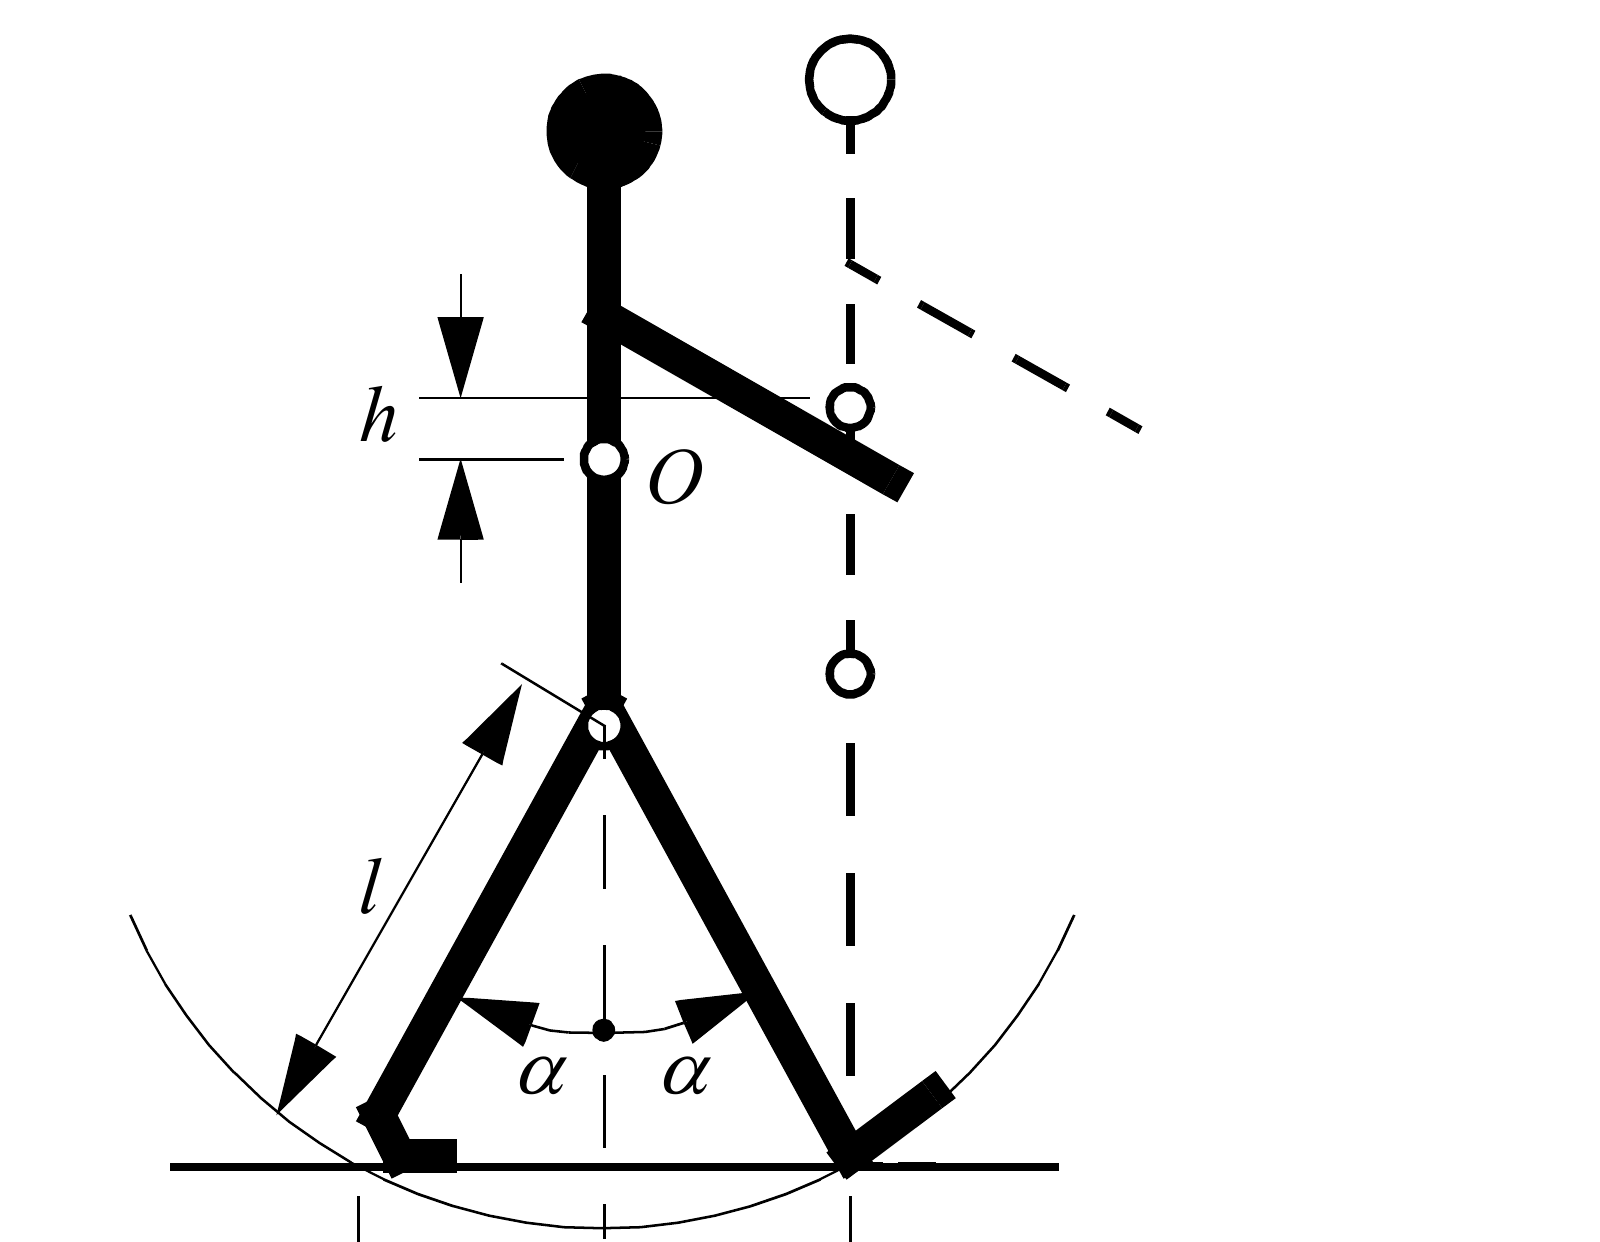
\includegraphics[width=\linewidth,height=4.5cm,keepaspectratio]{polygon.png}
\caption{A rolling polygon approaches a wheel as $d\to0$.}
\end{figure}
Centre $O$; radius $l$; step $d$; vertical excursion $h$; $\alpha$: half the angle between supports.
 Which should we choose?
\end{frame}

\begin{frame}[t]{Three questions for any way of moving}
\small
\vspace{-3mm}
\begin{block}{1. Stability}
Contact number and geometry; centre of mass. Example: a narrow base can tip.
\end{block}
\vspace{3mm}
\begin{block}{2. Contact}
Contact shape, angle and friction. Example: a tyre needs traction to push.
\end{block}
\vspace{3mm}
\begin{block}{3. Environment}
Structure, hardness and medium. Example: sand deforms; a hard floor does not.
\end{block}
\par\vspace{2mm}\small Which matters most for a lunar rover? For a vacuum cleaner?
\end{frame}

\begin{frame}[t]{Wheel or leg: which is more efficient?}
\small
\vspace{-4mm}
\begin{columns}[T,onlytextwidth]
\begin{column}{.60\textwidth}
\centering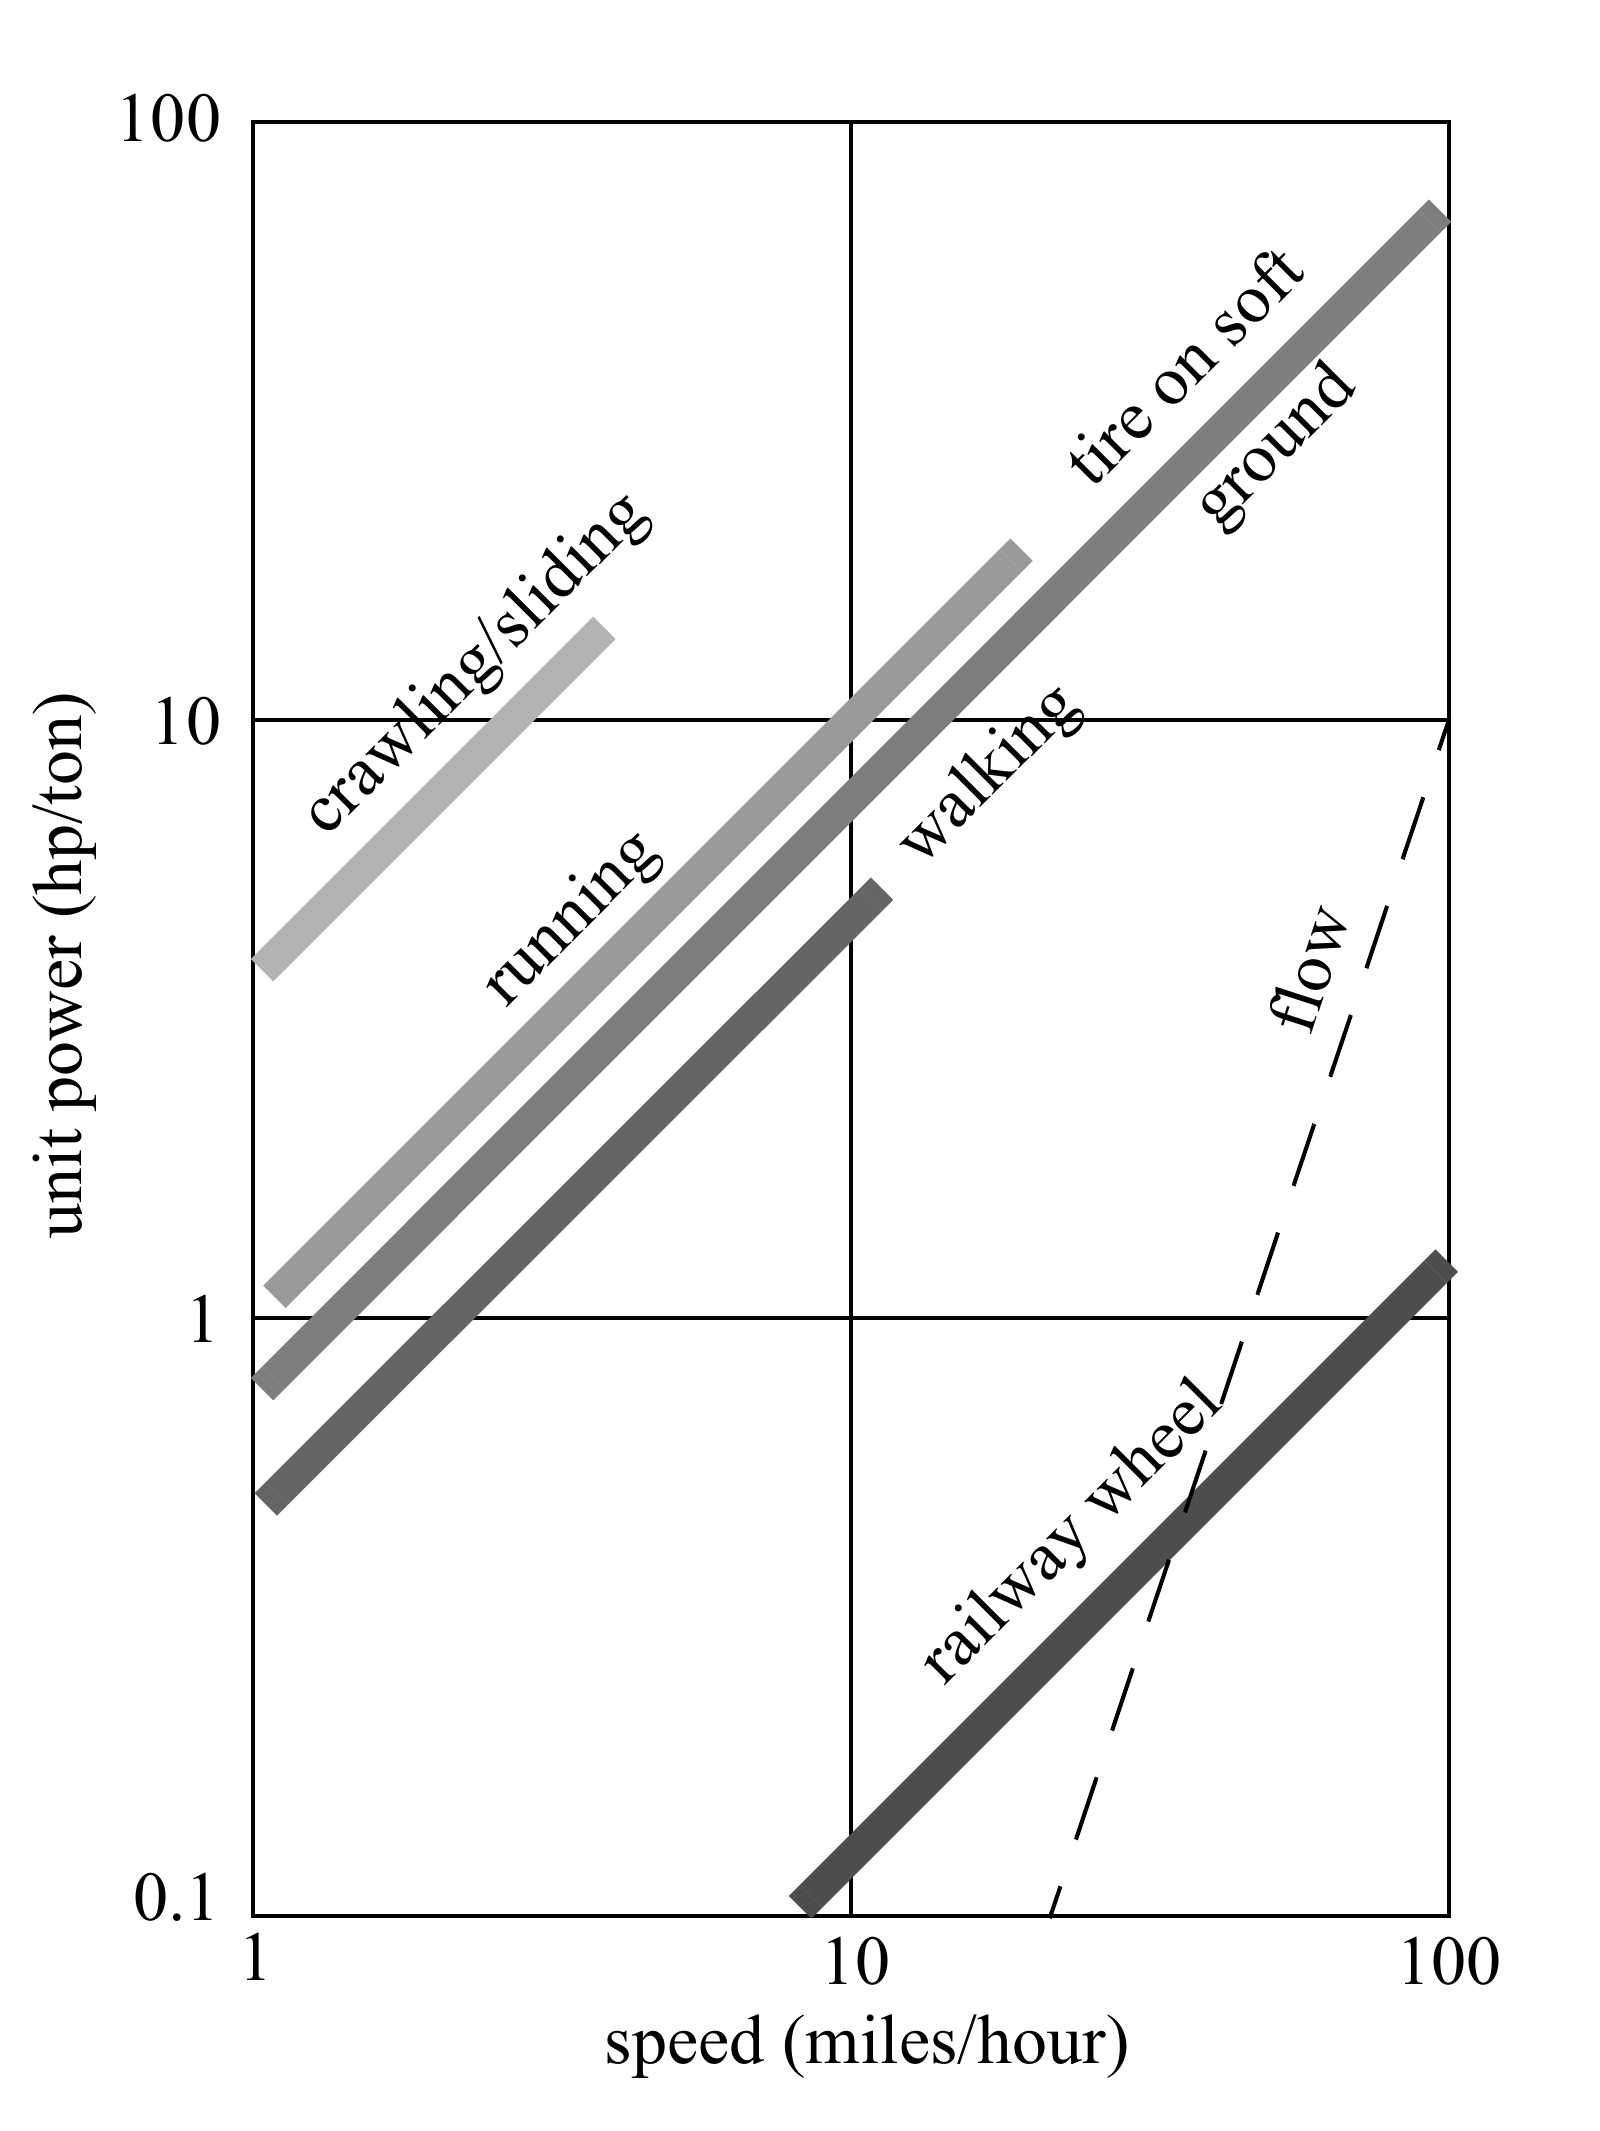
\includegraphics[width=\linewidth,height=6cm,keepaspectratio]{efficiency.png}
\end{column}
\begin{column}{.38\textwidth}
\vspace{8mm}
\textbf{Power per unit mass at each speed}
\par\vspace{4mm} On hard, flat ground the rail wheel needs 1--2 orders of magnitude less power than walking or running; soft ground raises tyre losses.
\par\vspace{4mm} Power per mass divided by speed is specific resistance: energy per weight and distance.
\par\vspace{5mm} Why build legs?
\end{column}
\end{columns}
\end{frame}

\begin{frame}[t]{Legs choose where to touch the ground}
\small
\vspace{-6mm}
\begin{columns}[T,onlytextwidth]\begin{column}{.49\textwidth}
\begin{figure}[H]\centering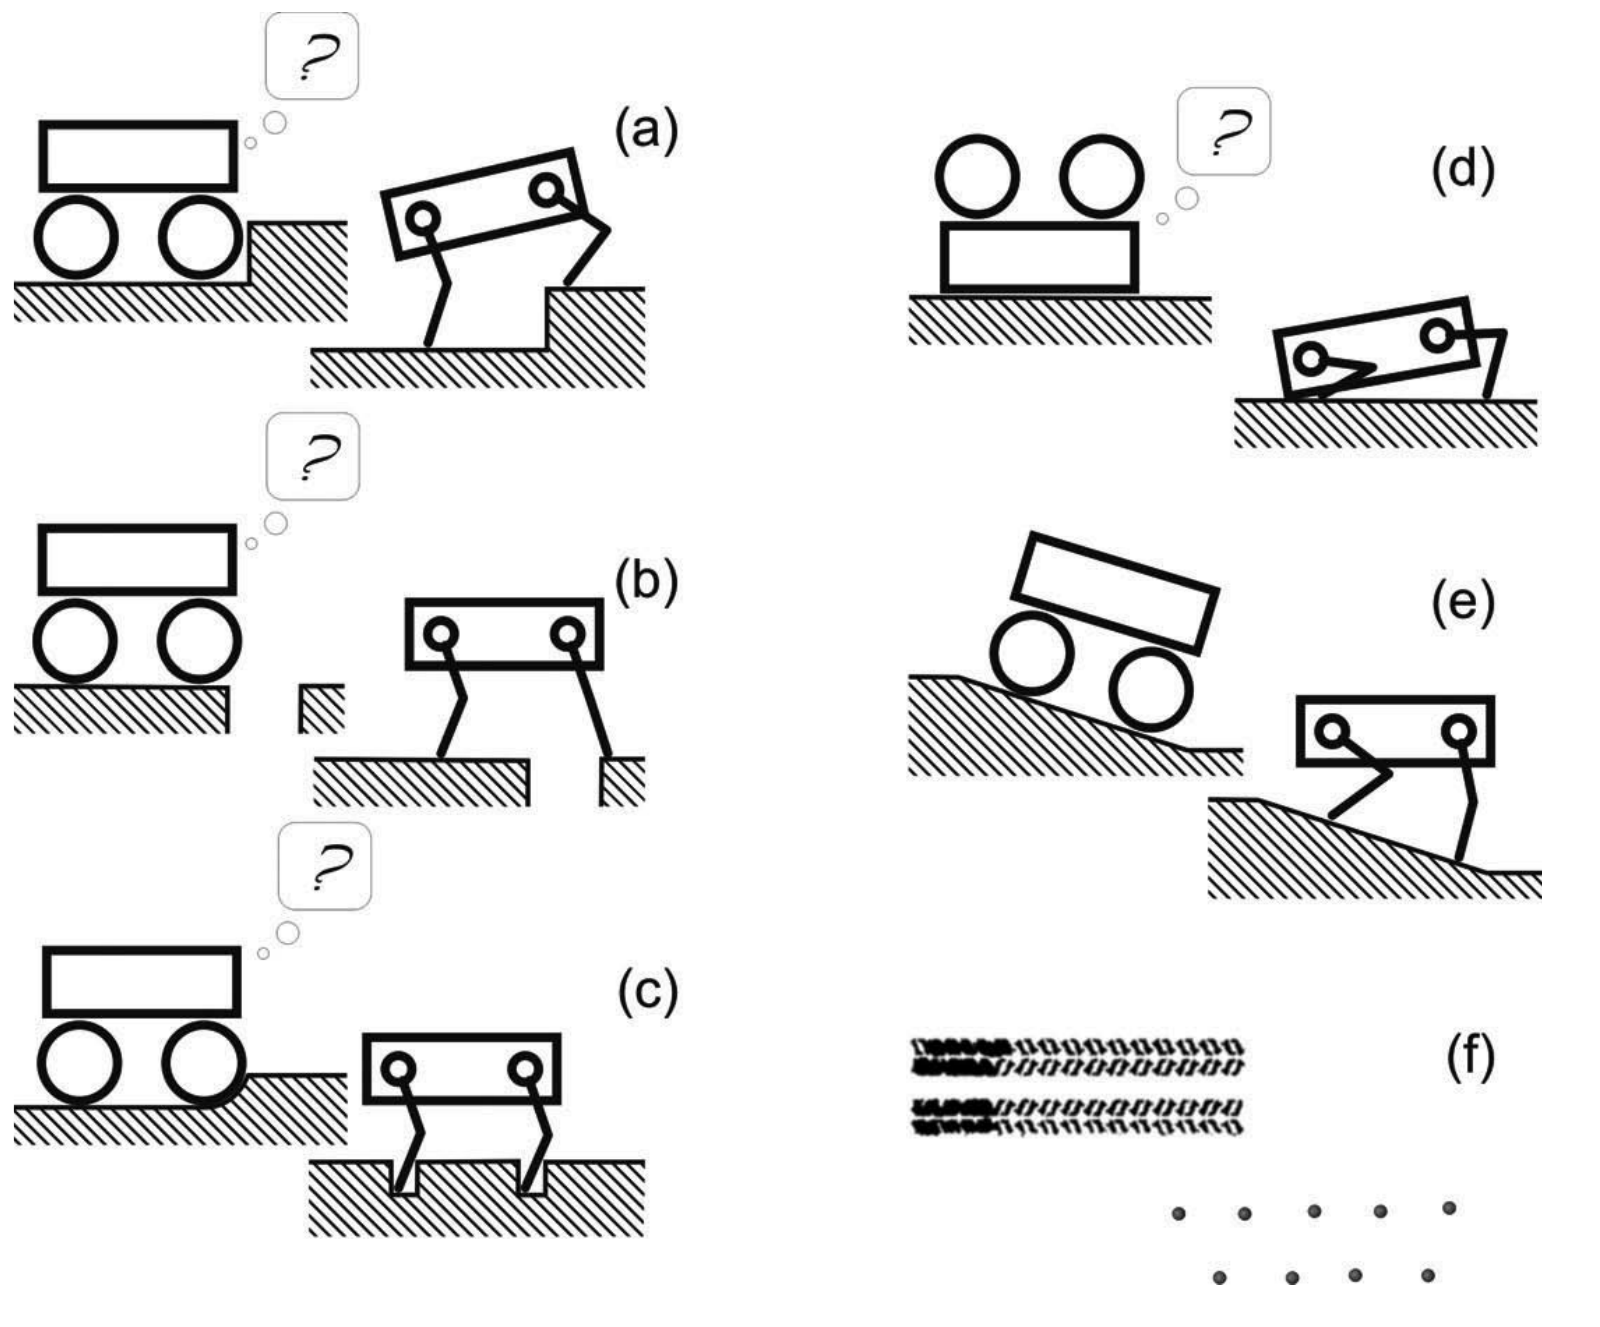
\includegraphics[width=\linewidth,height=4.5cm,keepaspectratio]{legs_benefits.png}
\caption{Legs use separate footholds.}
\end{figure}
\end{column}\begin{column}{.49\textwidth}
\begin{figure}[H]\centering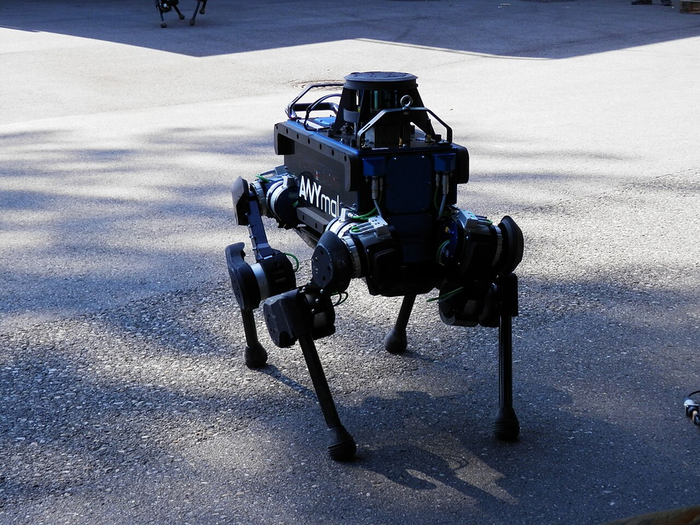
\includegraphics[width=\linewidth,height=4.5cm,keepaspectratio]{anymal.png}
\caption{A quadruped robot on rough ground.}
\end{figure}
\end{column}\end{columns}\small Legs can level the body and recover after a fall; wheels need continuous support.
\par\vspace{2mm}\small What do these capabilities cost?
\end{frame}

\begin{frame}[t]{What legs cost}
\small
\vspace{-6mm}
\begin{columns}[T,onlytextwidth]\begin{column}{.49\textwidth}
\begin{figure}[H]\centering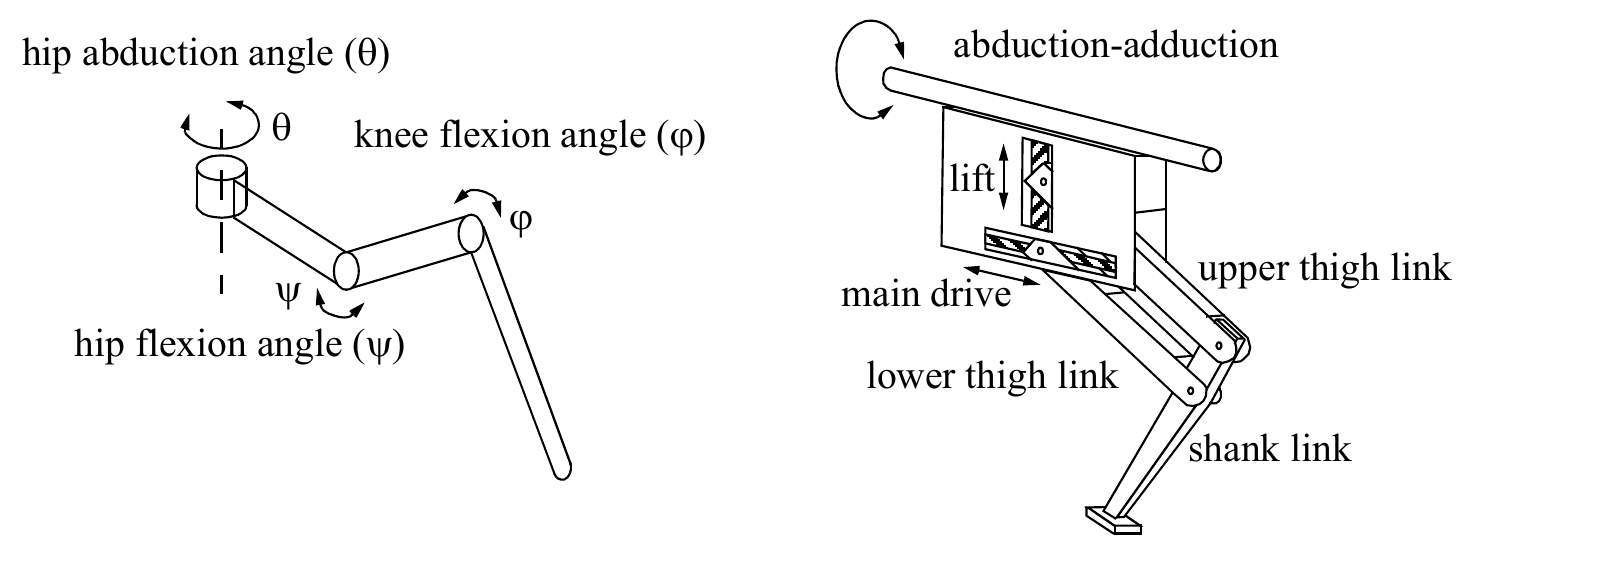
\includegraphics[width=\linewidth,height=4.5cm,keepaspectratio]{leg_dof.png}
\caption{Two legs with three independent joint motions each.}
\end{figure}
\end{column}\begin{column}{.49\textwidth}
\begin{block}{Degrees of freedom (DoF)}
DoF: one independent joint motion. Lifting and swinging usually needs two; three improve placement.
\end{block}
\vspace{2mm}
\begin{itemize}
\item More actuators: more mass and control.
\item Legs must accelerate their own mass.
\item Contact and balance need coordination.
\end{itemize}
\end{column}\end{columns}
\par\vspace{2mm}\small How many legs are needed just to stand?
\end{frame}

\begin{frame}[t]{How many legs are needed to stand?}
\small
\vspace{-6mm}
\begin{columns}[T,onlytextwidth]\begin{column}{.60\textwidth}
\begin{figure}[H]\centering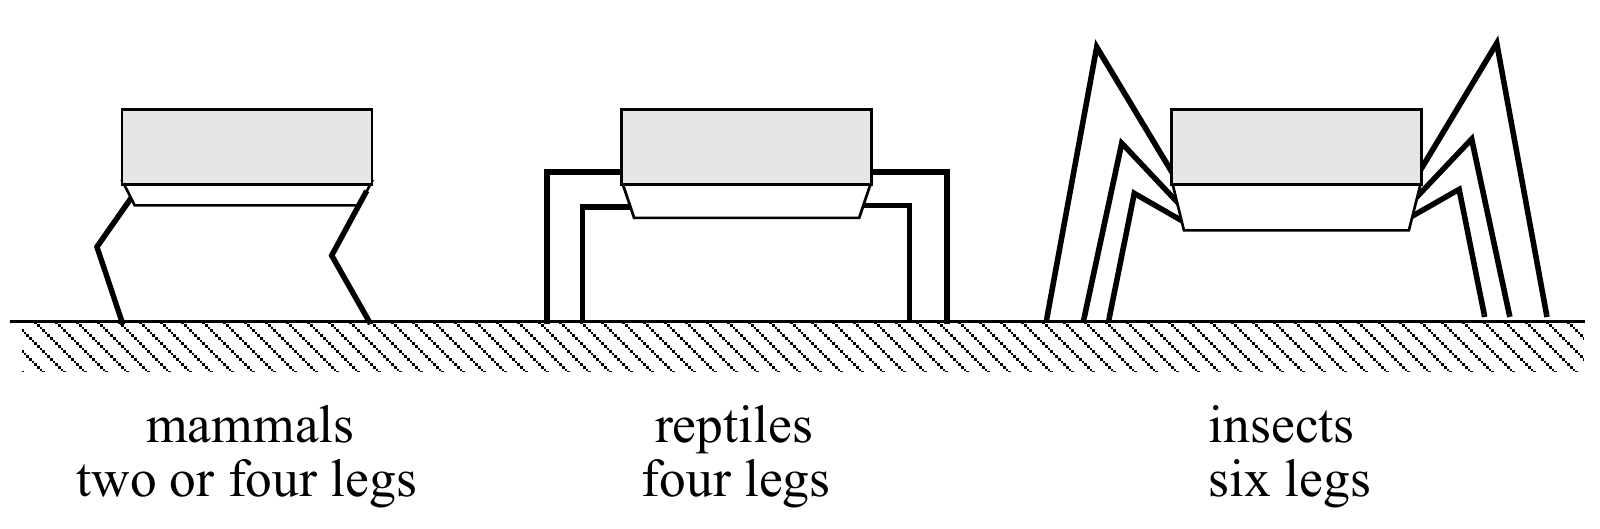
\includegraphics[width=\linewidth,height=4.5cm,keepaspectratio]{leg_animals.png}
\caption{Two, four and six legs.}
\end{figure}
\end{column}\begin{column}{.38\textwidth}
\centering\begin{tikzpicture}[scale=1.15,>=Latex,every node/.style={font=\small,align=center}]
\fill[blue!12] (0,0)--(3,0)--(1.5,2)--cycle;\draw[thick] (0,0)--(3,0)--(1.5,2)--cycle;\foreach \x/\y in {0/0,3/0,1.5/2}{\fill (\x,\y) circle (3pt);}\fill[blue] (1.5,.7) circle (3pt) node[right] {CoM projection};
\end{tikzpicture}\par\small Support polygon: the convex hull of ground contacts. CoM means centre of mass.
\end{column}\end{columns}\small With point contacts on level ground, three non-collinear contacts can support static balance. Four legs let one lift; six can alternate supporting tripods. Finite feet can provide a wider support region.
\par\vspace{2mm}\small Is staying inside that region the only way to balance?
\end{frame}

\begin{frame}[t]{Static, quasi-static and dynamic walking}
\footnotesize
\vspace{0mm}
\begin{columns}[T,onlytextwidth]\begin{column}{.49\textwidth}
\begin{block}{Static}
Freeze it: it stays up. The CoM projection stays in the support polygon.
\end{block}
\vspace{1.5mm}
\begin{block}{Quasi-static}
Move slowly; neglect inertia. Keep the CoM projection in the support polygon.
\end{block}
\vspace{1.5mm}
\begin{block}{Dynamic}
Freeze it: it falls. Motion and the next landing maintain balance.
\end{block}

\end{column}\begin{column}{.49\textwidth}
\centering\begin{tikzpicture}[>=Latex,every node/.style={font=\small,align=center}]

\foreach \y/\s in {0/Static,-1.5/Quasi-static}{\draw (-.3,\y)--(2.7,\y);\draw[thick] (.3,\y)--(1,\y+1)--(1.7,\y);\fill[blue] (1,\y+1) circle (3pt);\node[right] at (2.7,\y+.5) {\s};}\draw (-.3,-3)--(3,-3);\draw[thick] (.3,-3)--(2,-2)--(1.7,-3);\fill[blue] (2,-2) circle (3pt);\draw[dashed,blue] (2,-2)--(2,-3);\draw[dashed,thick] (2,-2)--(2.8,-3);\node[right] at (2.7,-2.5) {Dynamic};
\draw[->,blue] (1,-.5)--(1.5,-.5);\draw[->,blue,thick] (2,-2)--(2.6,-2);\draw[dashed] (1,1)--(1,0);

\end{tikzpicture}\par\footnotesize Tripod hexapod: static. Atlas and MIT Cheetah: dynamic. Dynamic movement enables running and jumping.
\end{column}\end{columns}
\end{frame}

\begin{frame}[t]{Video break: static versus dynamic}
\small
\vspace{-2mm}
\href{https://www.youtube.com/watch?v=RLxne70q6Fo}{\large Hexapod Walking Test -- Tripod, Wave \& Ripple Gaits}
\par{\footnotesize\url{https://www.youtube.com/watch?v=RLxne70q6Fo}}
\par How many legs touch the ground?
\par\vspace{3mm}
\href{https://www.youtube.com/watch?v=e2Q2Lx8O6Cg}{\large Steve Collin's Passive Dynamic Robot}
\par{\footnotesize\url{https://www.youtube.com/watch?v=e2Q2Lx8O6Cg}}
\par No motors: watch it walk down a slope.
\par\vspace{3mm}
\href{https://www.youtube.com/watch?v=LikxFZZO2sk}{\large Parkour Atlas}
\par{\footnotesize\url{https://www.youtube.com/watch?v=LikxFZZO2sk}}
\par When are both feet off the ground?
\par\vspace{3mm} How is the order of leg movements chosen?
\end{frame}

\begin{frame}[t]{Gait: the order in which legs move}
\footnotesize
\vspace{-1mm}
\begin{columns}[T,onlytextwidth]\begin{column}{.49\textwidth}
\begin{figure}[H]\centering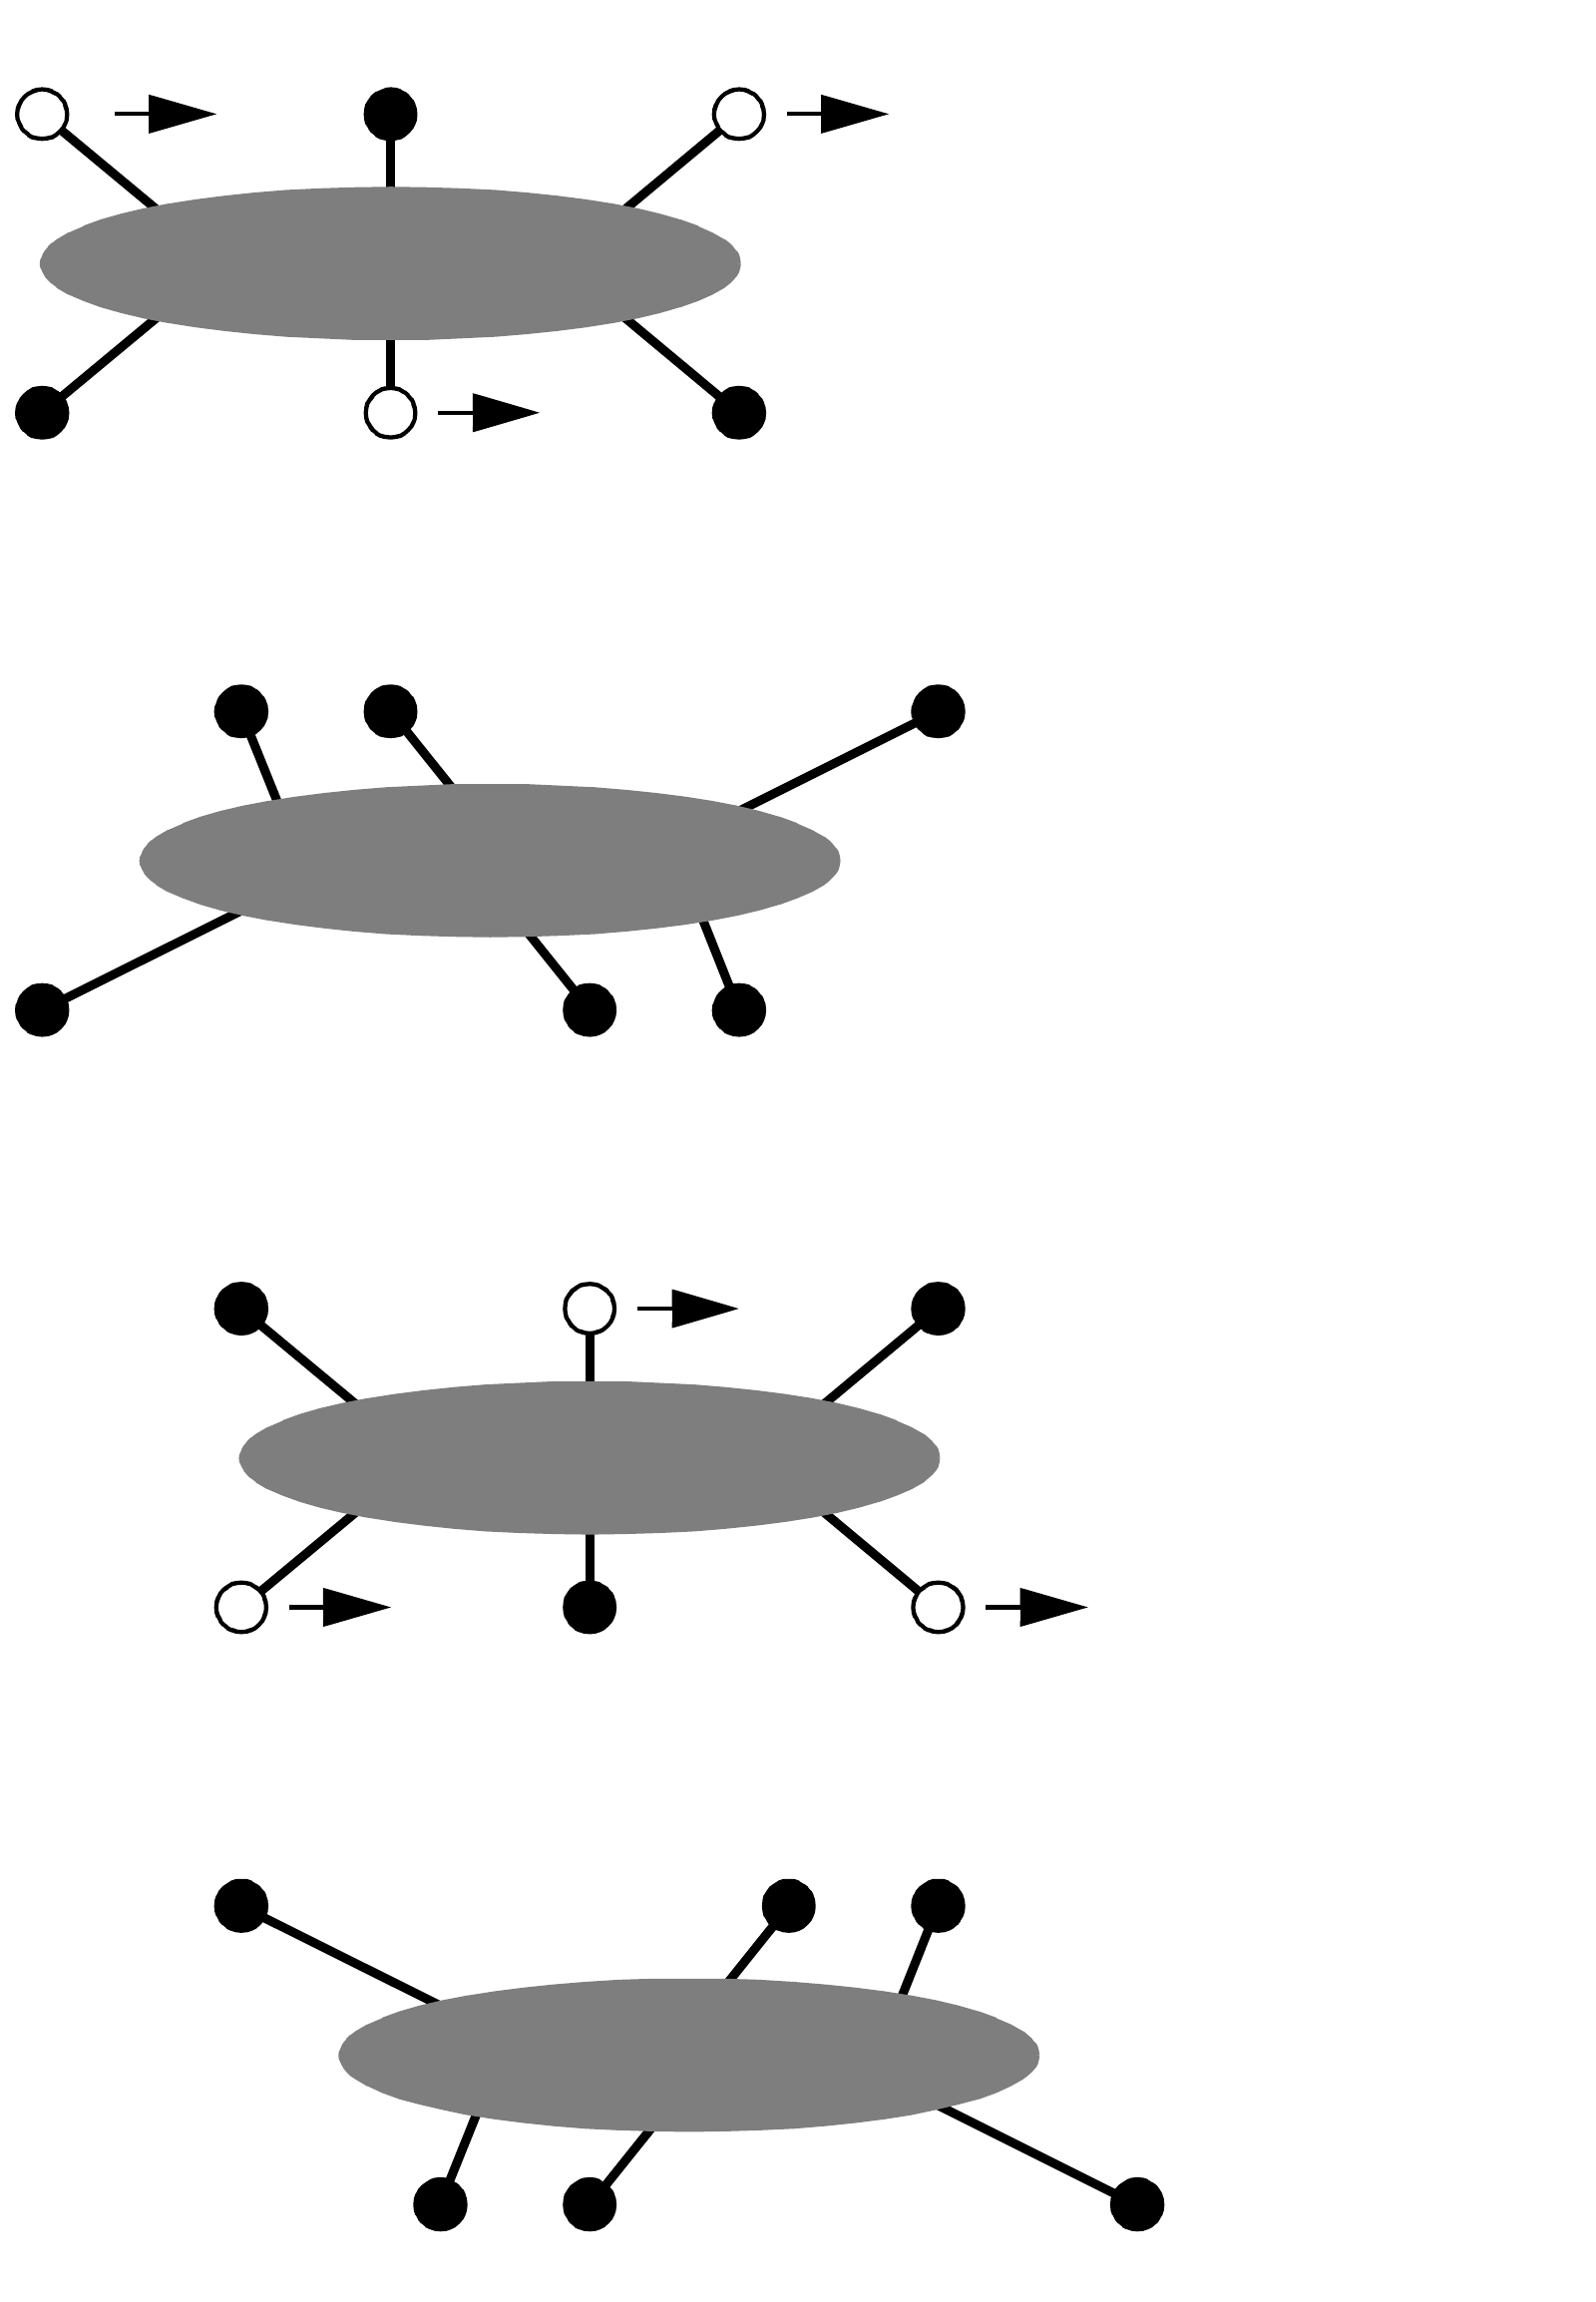
\includegraphics[width=\linewidth,height=4.1cm,keepaspectratio]{tripod.png}
\caption{Alternating support tripods.}
\end{figure}
\end{column}\begin{column}{.49\textwidth}
\textbf{Gait}: a repeating sequence of foot lift and lower events.\par\vspace{2mm}
For $k$ legs, count cyclic event orders:\[N=(2k-1)!\]\footnotesize $k=2$: $N=6$.\\ $k=6$: $N=11!=39\,916\,800$.\\ Event orders need not be useful or stable.\par\vspace{2mm}\centering\begin{tikzpicture}[>=Latex,every node/.style={font=\footnotesize,align=center}]
\draw[->] (0,0)--(4,0) node[right] {time};\foreach \x/\s in {.3/lift,1.5/lower,2.7/lift}{\draw (\x,-.1)--(\x,.1);\node[above] at (\x,.1) {\s};}
\end{tikzpicture}
\end{column}\end{columns}
\par\vspace{2mm}\footnotesize Which orders are useful, and why?
\end{frame}

\begin{frame}[t]{Why different gaits exist: speed against stability}
\footnotesize
\vspace{-4mm}
\begin{columns}[T,onlytextwidth]\begin{column}{.49\textwidth}
\centering\begin{tikzpicture}[scale=1.25,>=Latex,every node/.style={font=\small,align=center}]

\draw[rounded corners] (0,0) rectangle (2,2.5);
\foreach \y/\a/\b in {.4/1/2,1.25/3/4,2.1/5/6}{\draw (-.6,\y)--(2.6,\y);\node[left] at (-.6,\y) {\a};\node[right] at (2.6,\y) {\b};}
\node at (1,-.7) {Wave: $1\to2\to3\to4\to5\to6$};

\end{tikzpicture}\par Five feet support the body while one moves: most stable, slowest.
\end{column}\begin{column}{.49\textwidth}
\centering\begin{tikzpicture}[scale=1.25,>=Latex,every node/.style={font=\small,align=center}]

\draw[rounded corners] (0,0) rectangle (2,2.5);
\foreach \x/\y/\s in {-.6/.4/1,2.6/1.25/4,-.6/2.1/5}{\fill[blue] (\x,\y) circle (4pt);\node[above] at (\x,\y) {\s};}
\foreach \x/\y/\s in {2.6/.4/2,-.6/1.25/3,2.6/2.1/6}{\draw (\x,\y) circle (4pt);\node[above] at (\x,\y) {\s};}
\node at (1,-.7) {Tripod: $\{1,4,5\}\leftrightarrow\{2,3,6\}$};

\end{tikzpicture}\par Fastest of the three static hexapod gaits; ripple lies between wave and tripod.
\end{column}\end{columns}\par\medskip\footnotesize Quadruped trot alternates diagonal pairs; bound alternates front and rear pairs. Speed, terrain and energy favour different gaits.
 What makes each step expensive, and how can legs recover energy?
\end{frame}

\begin{frame}[t]{Why walking is expensive and how legs save energy}
\small
\vspace{-6mm}
\begin{columns}[T,onlytextwidth]
\begin{column}{.61\textwidth}
\begin{figure}[H]\centering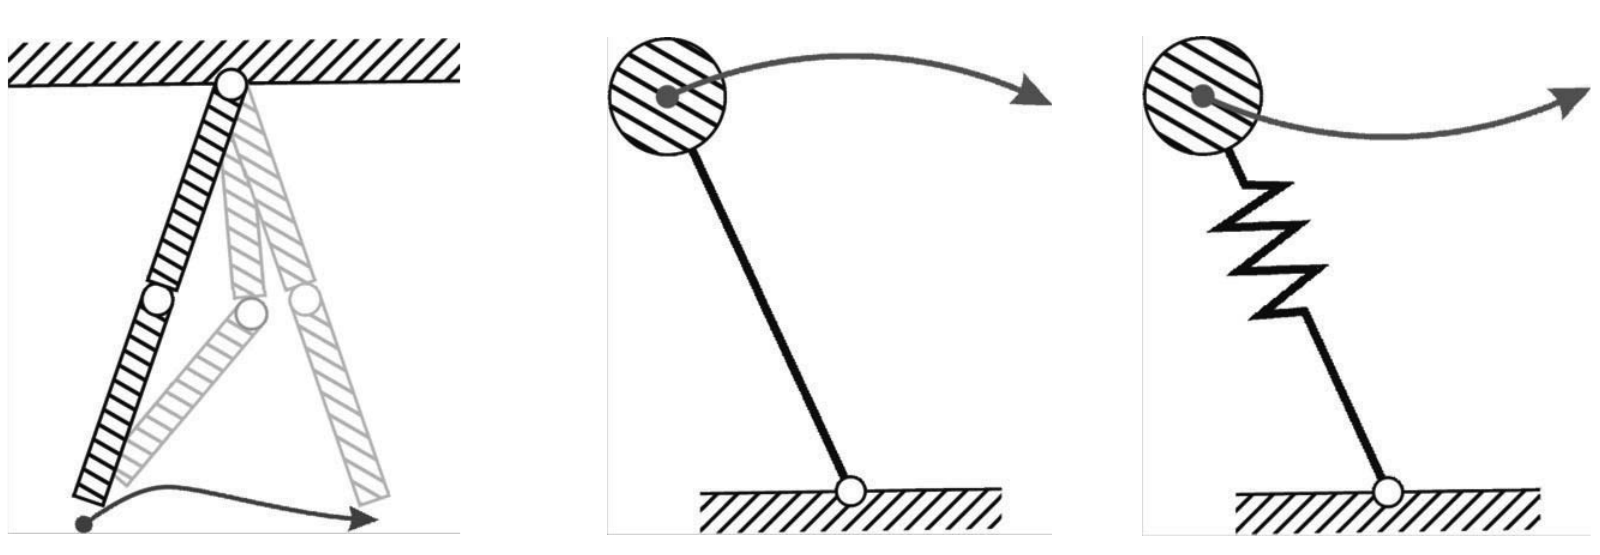
\includegraphics[width=\linewidth,height=4.5cm,keepaspectratio]{pendulum.png}
\caption{Swing: double pendulum. Stance: inverted pendulum. Running: spring.}
\end{figure}
\par\vspace{-2mm}\footnotesize
\textbf{Cost of transport}: energy per weight and distance (dimensionless). Each step accelerates and brakes legs; negative work is not fully recovered. Passive walkers use gravity and body dynamics; springs return landing energy.
\end{column}
\begin{column}{.37\textwidth}
\begin{figure}[H]\centering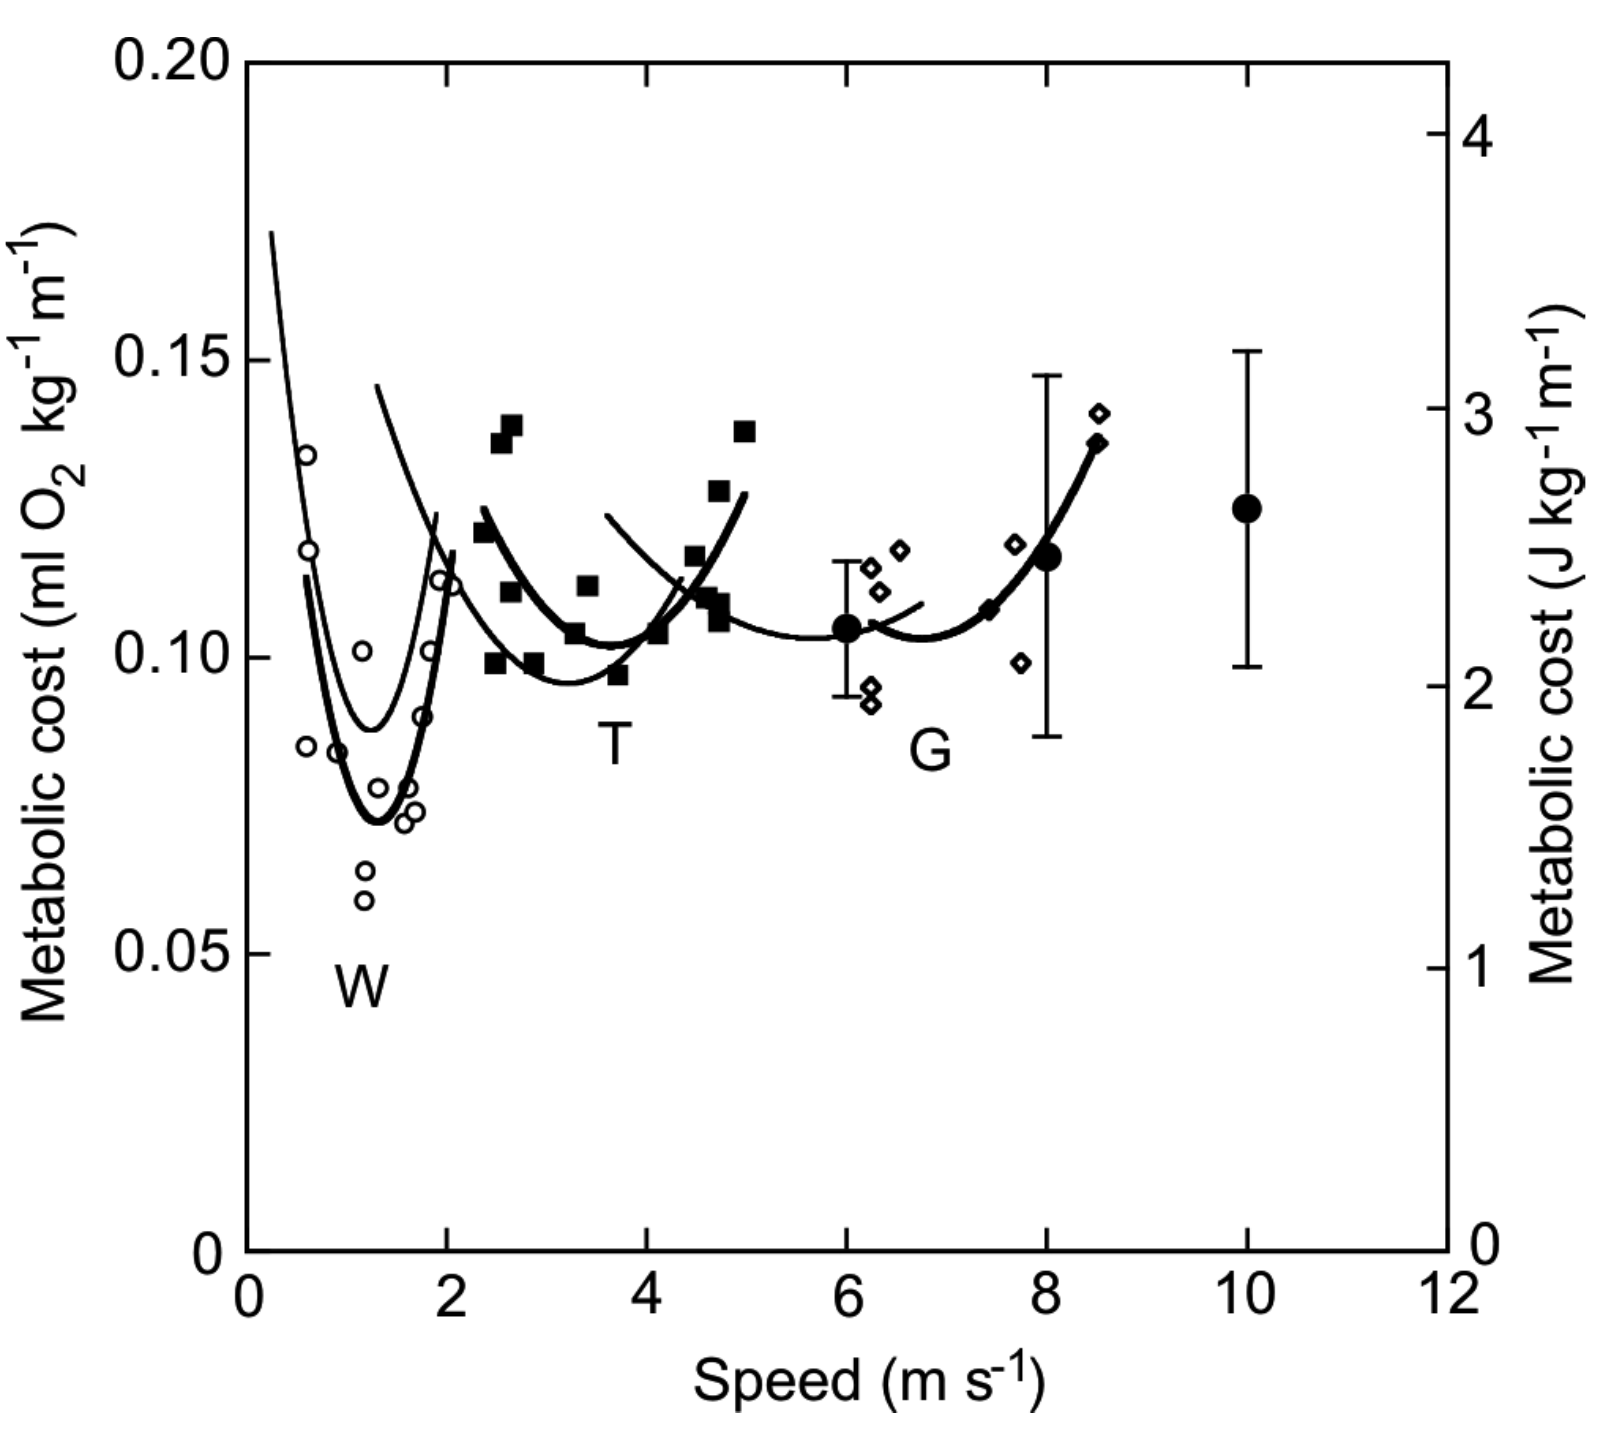
\includegraphics[width=\linewidth,height=4.5cm,keepaspectratio]{horse_cost.png}
\caption{Metabolic cost: walk (W), trot (T), gallop (G).}
\end{figure}
\par\vspace{-4mm}\footnotesize Who first used these ideas?
\end{column}
\end{columns}
\end{frame}

\begin{frame}[t]{History 1: Raibert's hopper (1983)}
\small
\vspace{0mm}
\begin{columns}[T,onlytextwidth]\begin{column}{.49\textwidth}
\begin{figure}[H]\centering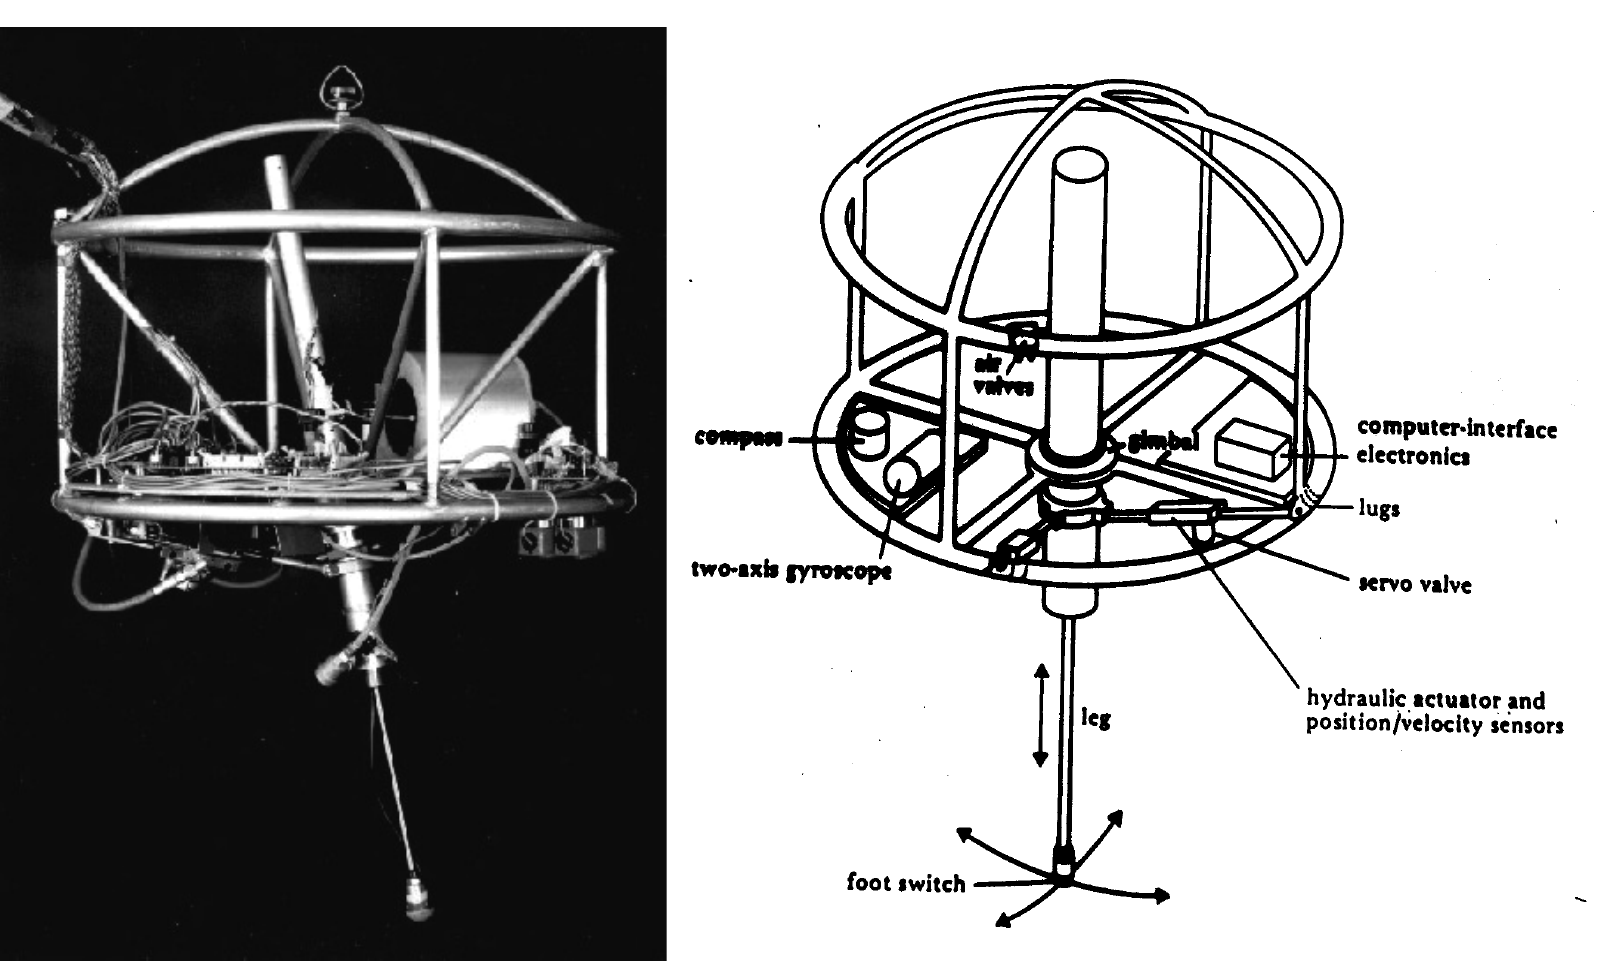
\includegraphics[width=\linewidth,height=4.5cm,keepaspectratio]{raibert.png}
\caption{The Raibert hopper.}
\end{figure}
\end{column}\begin{column}{.49\textwidth}
\begin{block}{One leg, active balance}
The robot cannot stand statically on a point foot. It continually corrects body attitude and speed by changing the leg angle.
\end{block}
\vspace{2mm}
\small Hydraulic extension produces the next hop; an off-board pump supplies power. Forward speed is controlled through foot placement.
\end{column}\end{columns}
\par\vspace{2mm}\small Can legs instead be simple and robust?
\end{frame}

\begin{frame}[t]{History 2: RHex, simple legs that rotate (2001)}
\small
\vspace{-6mm}
\begin{columns}[T,onlytextwidth]\begin{column}{.49\textwidth}
\begin{figure}[H]\centering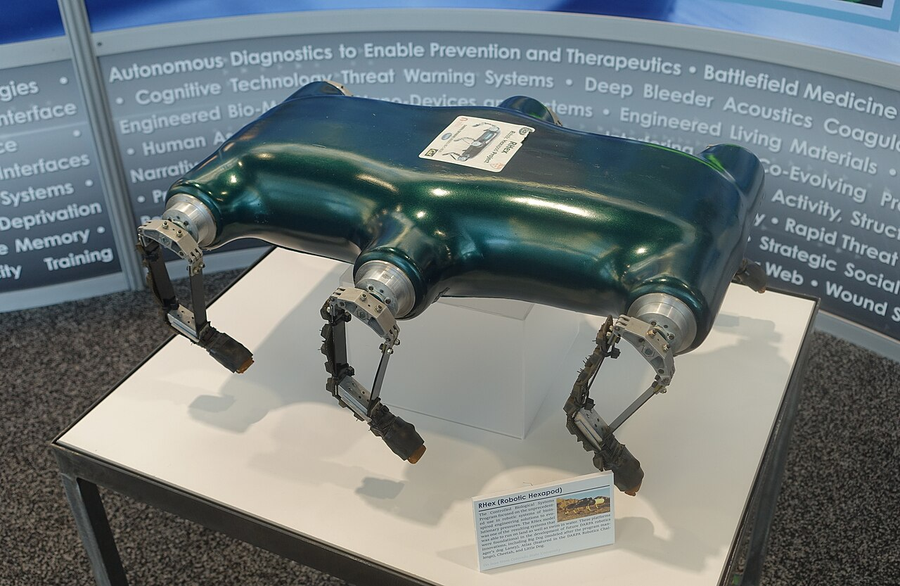
\includegraphics[width=\linewidth,height=4.5cm,keepaspectratio]{rhex.png}
\caption{RHex, a six-legged robot.}
\end{figure}
\end{column}\begin{column}{.49\textwidth}
\begin{block}{Mechanical simplicity}
Six rotating legs; one actuator per leg. Alternating tripods produce rough-terrain motion.
\end{block}
\vspace{2mm}
\small Research behaviours ran mostly open-loop, on a clock with little sensing. Toe slip on sand and rubble limits prediction.\par\medskip No clear single reason for its commercial follow-up history is established; a commercial version did exist.
\end{column}\end{columns}
\par\vspace{2mm}\small What changed with more articulated, actively controlled quadrupeds?
\end{frame}

\begin{frame}[t]{History 3: BigDog to Spot}
\footnotesize
\vspace{-6mm}
\begin{columns}[T,onlytextwidth]\begin{column}{.49\textwidth}
\begin{figure}[H]\centering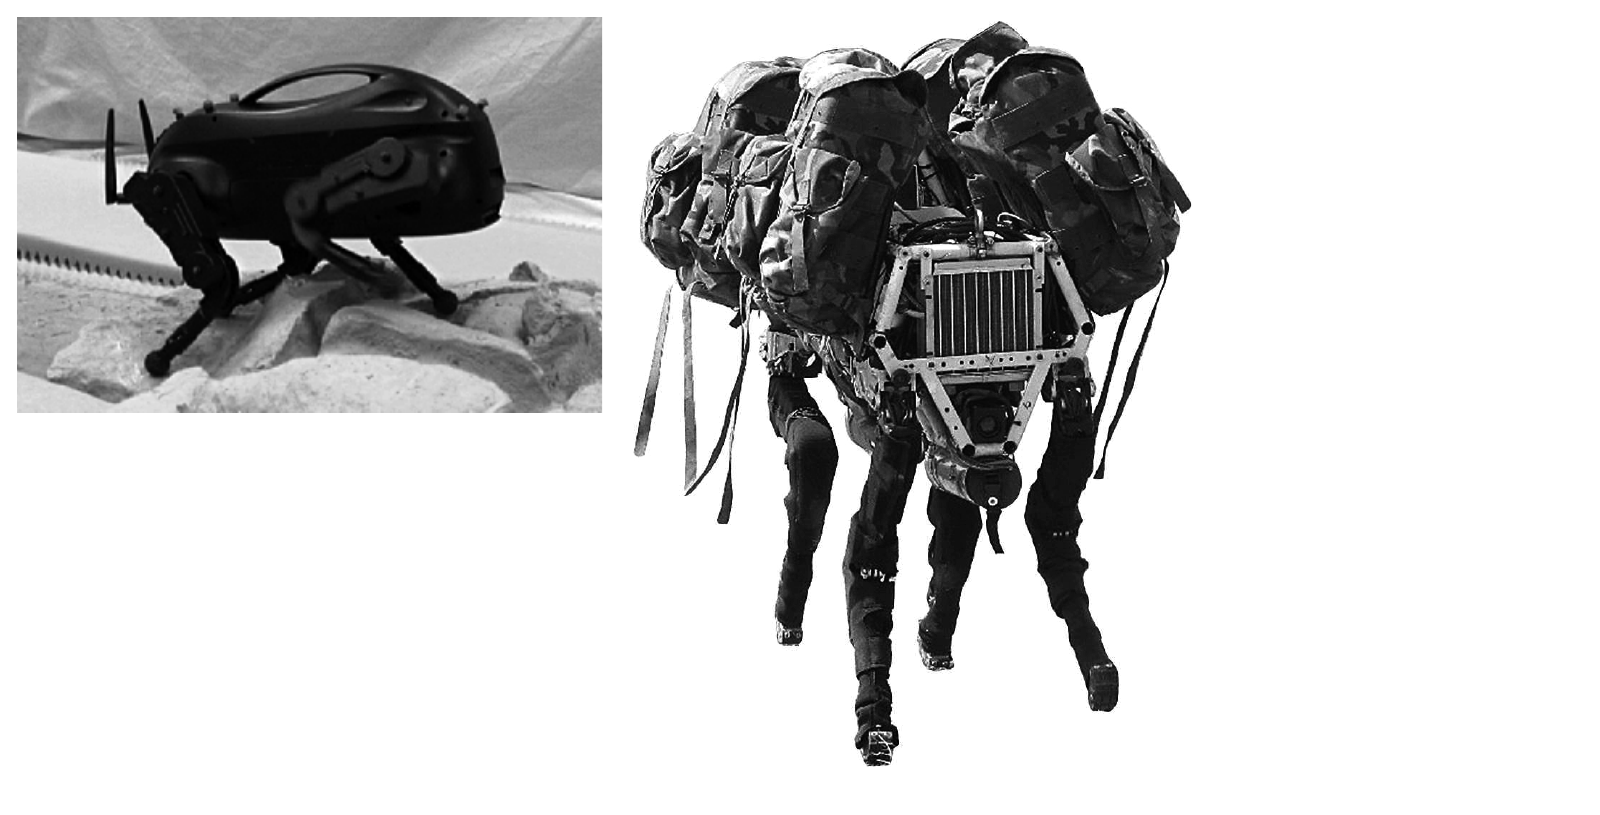
\includegraphics[width=\linewidth,height=4cm,keepaspectratio]{bigdog.png}
\caption{BigDog (2005): gasoline engine and hydraulics, about 150 kg payload; ended 2013 as too noisy.}
\end{figure}
\end{column}\begin{column}{.49\textwidth}
\begin{figure}[H]\centering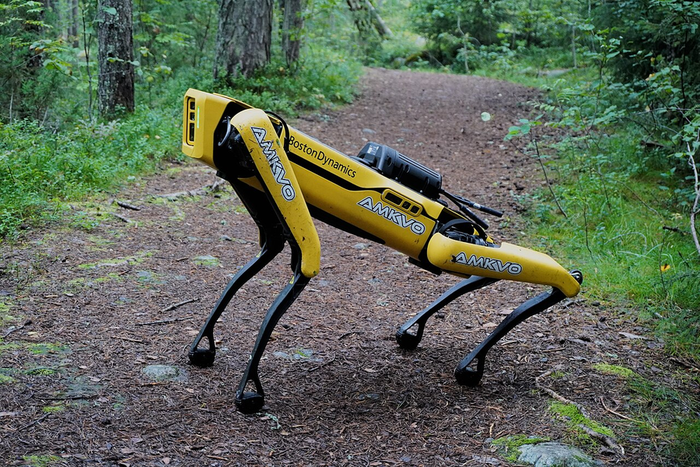
\includegraphics[width=\linewidth,height=4cm,keepaspectratio]{spot.png}
\caption{Spot: electric and quieter, about 20 kg payload; sold from 16 June 2020.}
\end{figure}
\end{column}\end{columns}
\footnotesize Engine-driven hydraulics brought noise and practical limits; Spot uses quieter electric drive. Quadrupeds are one branch. What about robots shaped like us?
\end{frame}

\begin{frame}[t]{History 4: humanoids}
\small
\vspace{-3mm}
\begin{block}{ASIMO}
Unveiled in November 2000; development stopped in 2018; retired from performing in March 2022. Controlled around a zero moment point (ZMP) criterion: balanced in motion.
\end{block}
\vspace{3mm}
\begin{block}{Atlas}
Hydraulic Atlas: 2013. Electric Atlas: April 2024. Product version: 5 January 2026 at CES, the Consumer Electronics Show.
\end{block}
\vspace{3mm}
\small A human-shaped body raises the same balance and contact problems. Dynamic motion makes flight phases and controlled landings possible.
\par\vspace{2mm}\small What documented changes connect these machines?
\end{frame}

\begin{frame}[t]{Why the field moved: what changed}
\small
\vspace{-2mm}
\begin{columns}[T,onlytextwidth]
\begin{column}{.42\textwidth}
\centering
\begin{tikzpicture}[>=Latex,every node/.style={font=\Large,anchor=west}]
\draw[->,thick] (0,.3)--(0,-4.6);
\foreach \y/\event in {0/{1983 --- Hopper},-1/{2001 --- RHex},-2/{2005 --- BigDog},-3/{2020 --- Spot},-4/{2026 --- Atlas}}{
\fill[blue] (0,\y) circle (2pt);
\node at (.2,\y) {\event};
}
\end{tikzpicture}
\end{column}
\begin{column}{.56\textwidth}
\begin{block}{Documented changes: actuation}
Engine-driven hydraulics to electric drive: less noise.
\end{block}
\vspace{3mm}
\begin{block}{Documented changes: control}
Clock-driven behaviours to feedback-controlled dynamic motion.
\end{block}
\vspace{3mm}
\begin{block}{Documented changes: commercial products}
Spot in 2020; product Atlas in 2026.
\end{block}
\end{column}
\end{columns}
\par\vspace{2mm} What else can robots learn from animals?
\end{frame}

\begin{frame}[t]{Biomimetic robots 1: running and jumping}
\footnotesize
\vspace{0mm}
\begin{columns}[T,onlytextwidth]\begin{column}{.49\textwidth}
\centering\resizebox{!}{3.5cm}{\begin{tikzpicture}[>=Latex,every node/.style={font=\small,align=center}]
\draw[very thick] (0,1)--(3,1);\draw[thick] (0,1)--(-.4,.5)--(.2,0);\draw[thick] (2.5,1)--(3.2,.5)--(2.8,0);\draw[->,blue] (0,1.8)--(3,1.8);\node at (1.5,-.5) {Running and obstacle clearance};
\end{tikzpicture}}\par\vspace{0mm}\begin{block}{MIT Cheetah (2015)}
Electric actuators; onboard laser ranging. Ran and jumped autonomously over obstacles up to about 46 cm at about 8 km/h.
\end{block}

\end{column}\begin{column}{.49\textwidth}
\centering\resizebox{!}{3.5cm}{\begin{tikzpicture}[>=Latex,every node/.style={font=\small,align=center}]
\draw[thick] (0,0)--(0,.4)--(.2,.6)--(-.2,.8)--(.2,1)--(0,1.2)--(0,1.5);\draw (0,1.7) circle (.2);\draw[->,blue,thick] (.7,.2) .. controls (2,2.8) .. (3,.2);\node at (1.5,-.5) {Spring-assisted jumping};
\end{tikzpicture}}\par\vspace{0mm}\begin{block}{Salto (2016)}
Galago-inspired; 100 g, 26 cm. Spring energy enables repeated jumps about 1 m high.
\end{block}

\end{column}\end{columns}
\par\vspace{0.5mm}\footnotesize Not all animals walk. What about crawling and climbing?
\end{frame}

\begin{frame}[t]{Biomimetic robots 2: crawling and climbing}
\footnotesize
\vspace{-3mm}
\begin{columns}[T,onlytextwidth]\begin{column}{.49\textwidth}
\centering\resizebox{!}{3.5cm}{\begin{tikzpicture}[>=Latex,every node/.style={font=\small,align=center}]
\draw[very thick,blue] plot[smooth] coordinates {(0,0)(.5,.5)(1,0)(1.5,-.5)(2,0)(2.5,.5)(3,0)};\foreach \x in {0,.5,1,1.5,2,2.5,3}{\draw (\x,-.7)--(\x,-.9);}\node at (1.5,-1.3) {Articulated body waves};
\end{tikzpicture}}\par\vspace{-2mm}\begin{block}{CMU modular snake}
Carnegie Mellon University: tethered, 16 modules; undulation and rolling. Deployed in a Mexico City earthquake building (September 2017); no survivors found.
\end{block}

\end{column}\begin{column}{.49\textwidth}
\centering\resizebox{!}{3.5cm}{\begin{tikzpicture}[>=Latex,every node/.style={font=\small,align=center}]
\draw[thick] (2,-.5)--(2,2);\draw[rounded corners] (.8,.5) rectangle (1.3,1.5);\foreach \y in {.6,1.4}{\draw (.8,\y)--(.3,\y+.3);\draw (1.3,\y)--(2,\y+.3);}\node at (1,-1) {Adhesion and controlled foot forces};
\end{tikzpicture}}\par\vspace{-2mm}\begin{block}{Stickybot}
Gecko-inspired directional dry adhesive. Layered compliance, directional adhesion and foot-force control; climbed glass and glazed tile at 4 cm/s.
\end{block}

\end{column}\end{columns}
\par\vspace{0.5mm}\footnotesize How does the environment change the design in water?
\end{frame}

\begin{frame}[t]{Biomimetic robots 3: swimming}
\footnotesize
\vspace{-2mm}

\centering\resizebox{!}{3.5cm}{\begin{tikzpicture}[>=Latex,every node/.style={font=\small,align=center}]
\draw[thick,blue] (0,0) .. controls (1,1) and (2,1) .. (3,0) .. controls (2,-1) and (1,-1) .. (0,0);\draw[thick,blue] (3,0)--(4,.7)--(4,-.7)--cycle;\fill (1,.2) circle (2pt);\draw[<->] (4.3,-.7)--(4.3,.7);\draw[->] (0,1.3)--(-.8,1.3);
\end{tikzpicture}}
\par\vspace{-3mm}
\begin{columns}[T,onlytextwidth]\begin{column}{.49\textwidth}
\begin{block}{SoFi: a soft robotic fish (2018)}
Undulates its tail to swim. Adjustable weight and a buoyancy control unit regulate depth.
\end{block}\end{column}\begin{column}{.49\textwidth}\begin{block}{Return to the three questions}
Water supports weight and provides reaction forces. Contact with a floor is no longer required.
\end{block}\end{column}\end{columns}

\footnotesize Tested at Rainbow Reef, Fiji: 40-minute dives to over 50 ft (about 15 m), near real fish without scaring them.

\par\vspace{2mm}\footnotesize Back on land, what can tracks and screws offer?
\end{frame}

\begin{frame}[t]{Tracks and screws}
\footnotesize
\vspace{-2mm}
\begin{columns}[T,onlytextwidth]\begin{column}{.54\textwidth}
\centering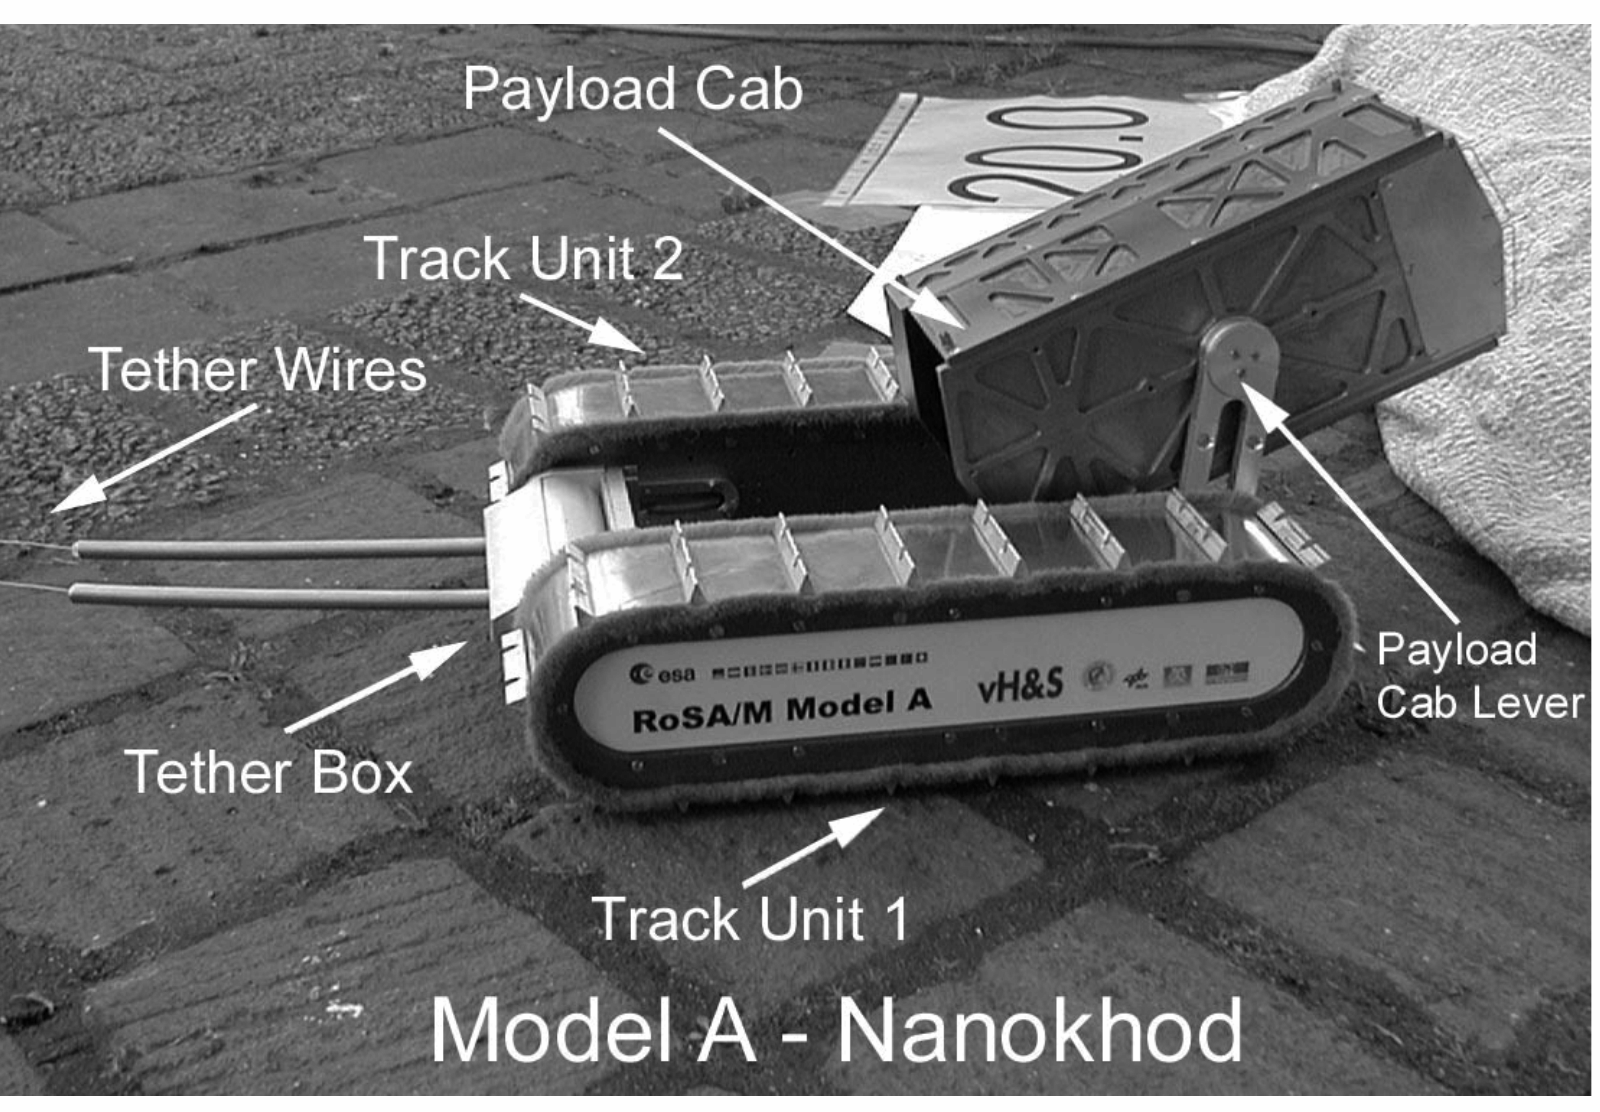
\includegraphics[width=\linewidth,height=5.4cm,keepaspectratio]{tracks.png}

\end{column}\begin{column}{.44\textwidth}
\centering\resizebox{!}{3.5cm}{\begin{tikzpicture}[>=Latex,every node/.style={font=\small,align=center}]

\draw[rounded corners,thick] (0,1) rectangle (3,2);
\foreach \y in {0,.6}{\draw[thick] (-.2,\y) rectangle (3.2,\y+.35);\foreach \x in {0,.5,1,1.5,2,2.5}{\draw[thick,blue] (\x,\y)--(\x+.4,\y+.35);}}
\node at (1.5,-.6) {Screw drums};

\end{tikzpicture}}\par\footnotesize Nanokhod is a tracked microrover. Tracks spread load over a large patch; turning requires skid. Terrain friction reduces odometry accuracy.
\end{column}\end{columns}
\par\vspace{2mm}\footnotesize Can we combine the advantages of wheels and legs?
\end{frame}

\begin{frame}[t]{Wheel-leg hybrids}
\small
\vspace{-2mm}
\begin{columns}[T,onlytextwidth]\begin{column}{.60\textwidth}
\begin{figure}[H]\centering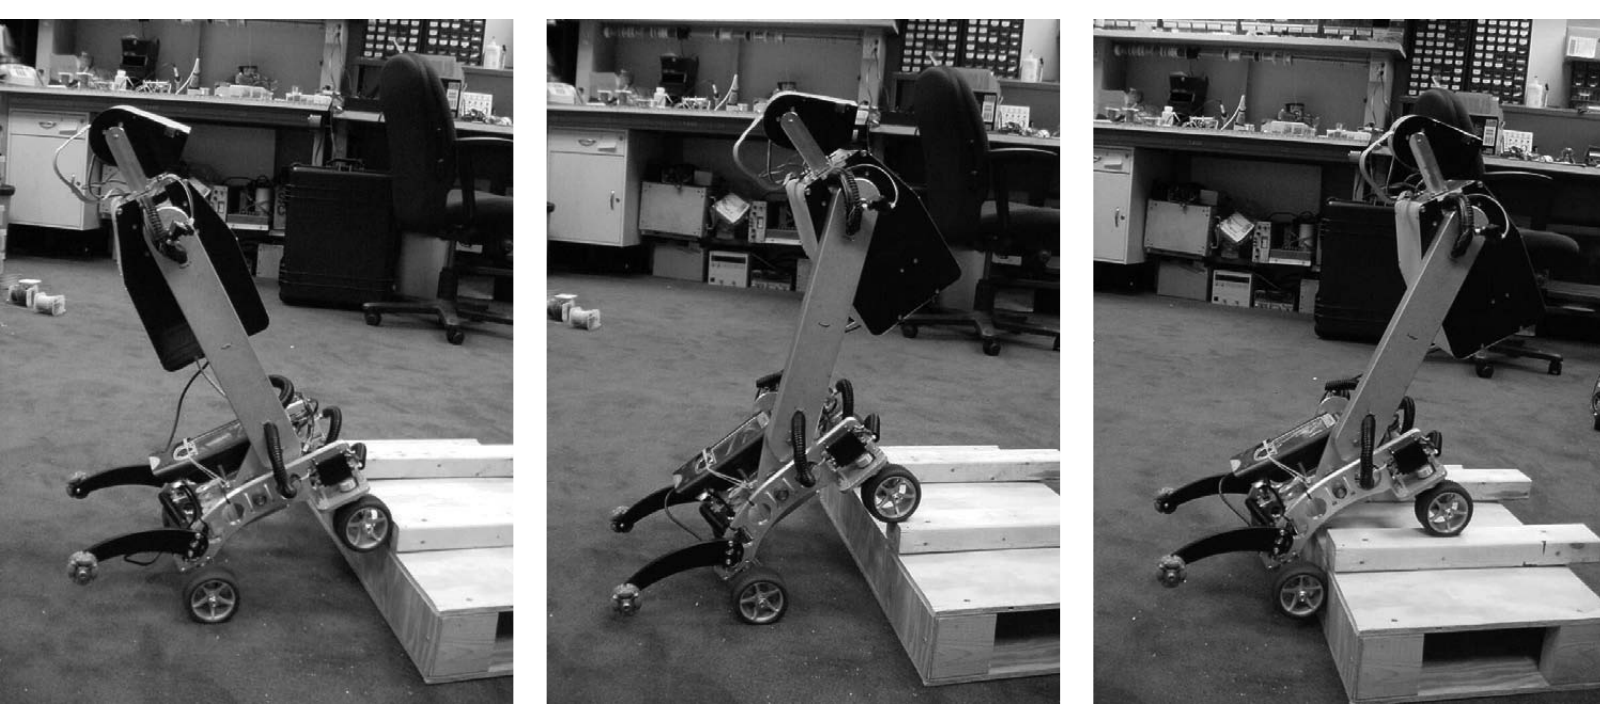
\includegraphics[width=\linewidth,height=4.5cm,keepaspectratio]{walking_wheels.png}
\caption{Personal Rover shifts its centre of mass to climb.}
\end{figure}
\end{column}\begin{column}{.38\textwidth}
\footnotesize
\begin{tabularx}{\linewidth}{lX}
\toprule Mechanism & Main trade-off\\\midrule
Legs & Footholds; swing losses\\
Tracks & Large patch; skid turns\\
Screws & Helical contact\\
Wheels & Efficient; continuous support\\
Hybrids & Adaptation; complexity\\\bottomrule
\end{tabularx}
\par\vspace{2mm} Rolling on level ground; weight shifting for ledges.

\end{column}\end{columns}
\par\vspace{2mm}\footnotesize Wheels dominate on flat ground. What wheel types exist?
\end{frame}

\begin{frame}[t]{Wheel types}
\small
\vspace{0mm}
\begin{columns}[T,onlytextwidth]
\begin{column}{.65\textwidth}
\centering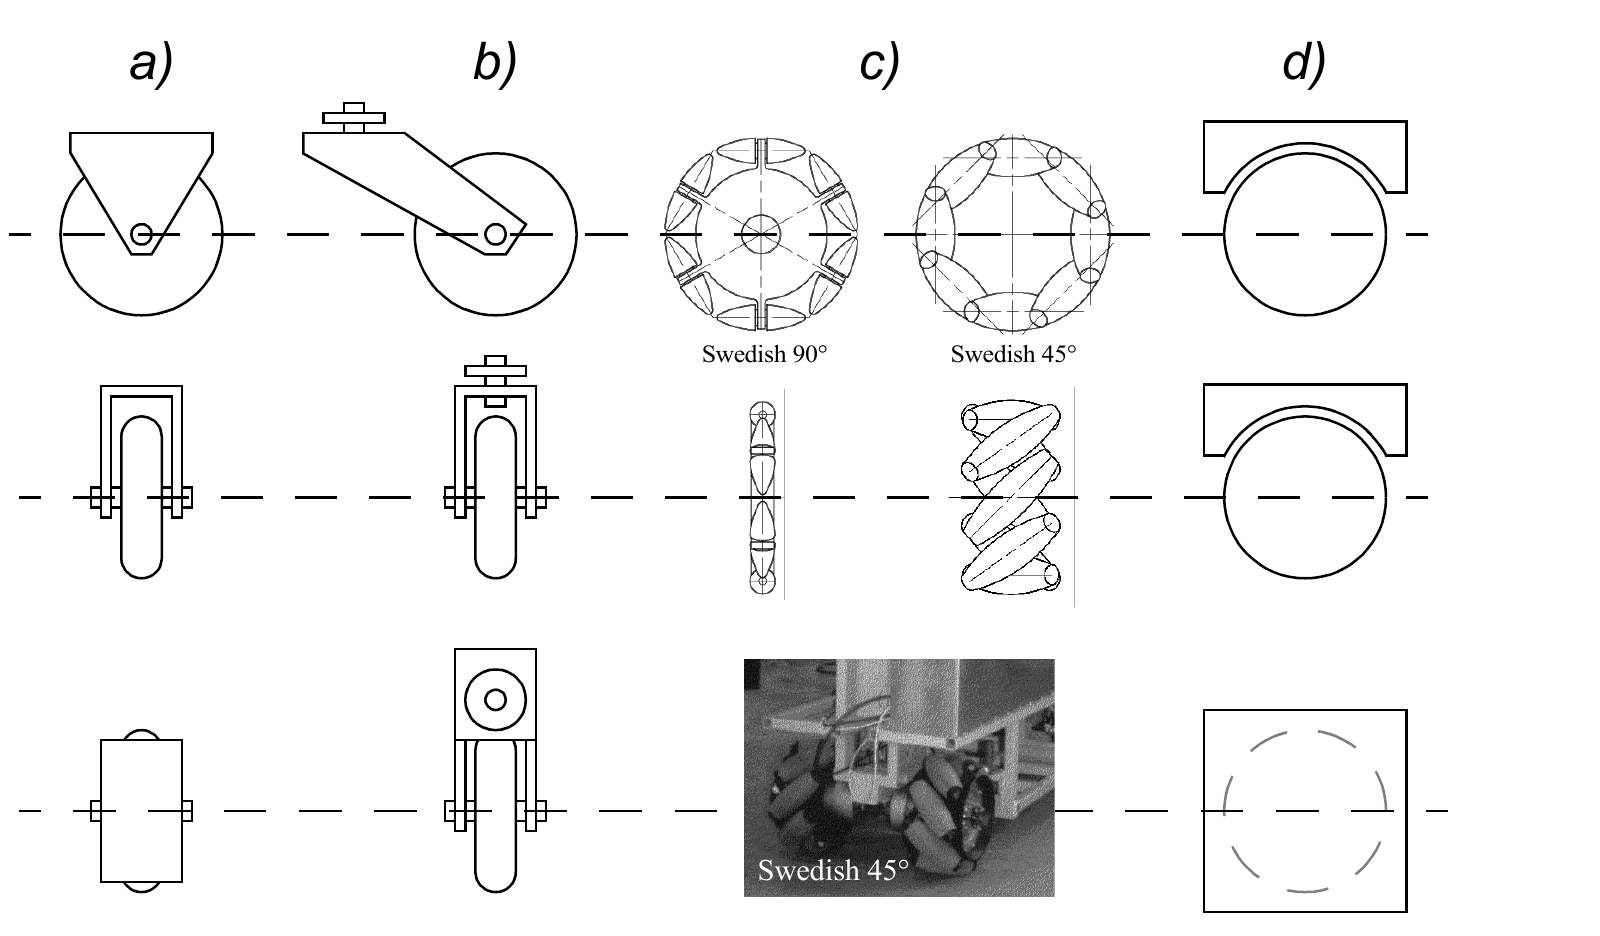
\includegraphics[width=\linewidth,height=6cm,keepaspectratio]{wheels.png}
\end{column}
\begin{column}{.33\textwidth}
\footnotesize
\textbf{Four wheel types}
\par\vspace{3mm}\textbf{Standard:} rolls forward; resists sideways motion. Fixed or actively steered.
\par\vspace{3mm}\textbf{Castor:} passive steering; axis offset from contact.
\par\vspace{3mm}\textbf{Swedish:} free rollers add a direction of motion.
\par\vspace{3mm}\textbf{Spherical:} a ball rolls in any direction.
\end{column}
\end{columns}
\par\vspace{2mm}\footnotesize How are wheels arranged on a robot?
\end{frame}

\begin{frame}[t]{Wheel arrangements}
\footnotesize
\vspace{-3mm}
\centering
\begin{tikzpicture}[scale=.93,>=Latex,every node/.style={font=\small,align=center}]
\begin{scope}[shift={(0,0)}]
\draw (0,-.6) rectangle (2,.6);\draw[very thick] (-.25,-.65)--(.25,-.65);\draw[very thick] (-.25,.65)--(.25,.65);\draw[very thick] (1.75,-.15)--(2.25,.15);
\node at (1,-1.3) {Tricycle\\fixed pair + steered};
\end{scope}
\begin{scope}[shift={(4,0)}]
\draw (0,-.6) rectangle (1.6,.6);\draw[very thick] (-.25,-.65)--(.25,-.65);\draw[very thick] (-.25,.65)--(.25,.65);\draw (1.3,0) circle (.18);
\node at (.8,-1.3) {Differential\\+ castor};
\end{scope}
\begin{scope}[shift={(8,0)}]
\draw (0,-.6) rectangle (2,.6);\draw[very thick] (-.25,-.65)--(.25,-.65);\draw[very thick] (-.25,.65)--(.25,.65);
\draw[very thick] (1.75,-.85)--(2.25,-.5);\draw[very thick] (1.75,.5)--(2.25,.8);
\node at (1,-1.3) {Ackermann\\linked steering};
\end{scope}
\begin{scope}[shift={(2,-3.2)}]
\draw (0,.7)--(-.7,-.5)--(.7,-.5)--cycle;
\foreach \x/\y/\a in {0/.7/0,-.7/-.5/60,.7/-.5/-60}{\begin{scope}[shift={(\x,\y)},rotate=\a]\draw[very thick,teal] (-.3,0)--(.3,0);\foreach \s in {-.2,0,.2}{\draw (\s-.06,-.1)--(\s+.06,.1);}\end{scope}}
\node at (0,-1.4) {Swedish\\free rollers};
\end{scope}
\begin{scope}[shift={(7,-3.2)}]
\draw (0,.7)--(-.7,-.5)--(.7,-.5)--cycle;
\foreach \x/\y in {0/.7,-.7/-.5,.7/-.5}{\draw[very thick,blue] (\x-.25,\y-.15)--(\x+.25,\y+.15);\draw[->] (\x+.25,\y+.3) arc (45:140:.25);}
\node at (0,-1.4) {Synchro drive\\linked drive / steering};
\end{scope}
\end{tikzpicture}
\par\footnotesize Differential: independent wheel speeds. Ackermann: linked front steering. Tricycle: one steered wheel. Omni: lateral motion. Synchro: linked drive and steering. Which keeps contact on uneven ground?
\end{frame}

\begin{frame}[t]{Stability on uneven ground}
\small
\vspace{-6mm}
\begin{columns}[T,onlytextwidth]\begin{column}{.49\textwidth}
\begin{figure}[H]\centering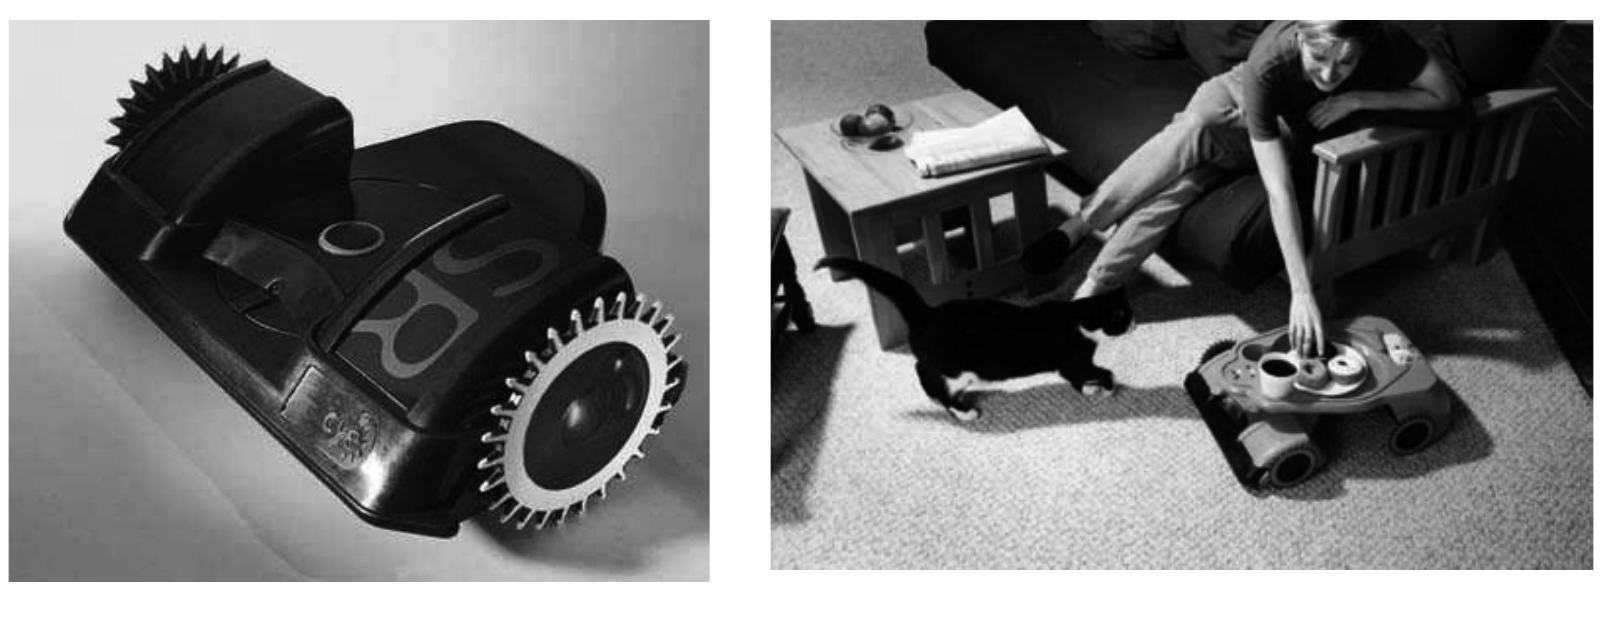
\includegraphics[width=\linewidth,height=4.5cm,keepaspectratio]{cye.png}
\caption{Cye: two wheels, low centre of mass.}
\end{figure}
\small Two wheels: CoM below axle. Three contacts: support triangle. More rigid supports need suspension on uneven ground.
\end{column}\begin{column}{.49\textwidth}
\begin{figure}[H]\centering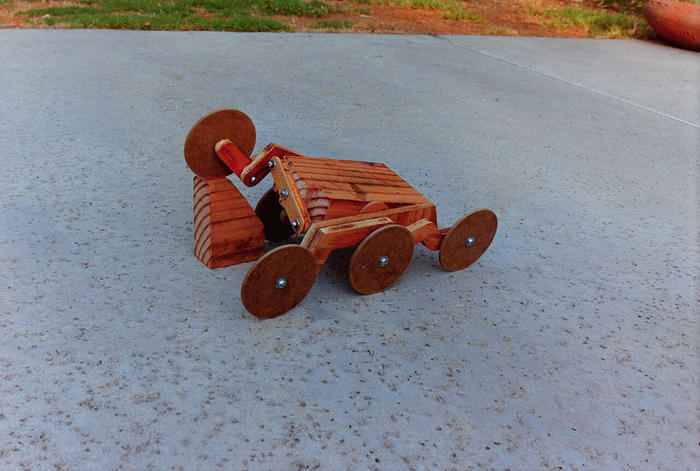
\includegraphics[width=\linewidth,height=4.5cm,keepaspectratio]{rocker_bogie.png}
\caption{A rocker-bogie suspension model.}
\end{figure}
\end{column}\end{columns}
\par\vspace{2mm}\small How do the locomotion choices compare?
\end{frame}

\begin{frame}[t]{Part A summary and the bridge}
\small
\vspace{0mm}
\begin{tabularx}{\linewidth}{lXXXX}
\toprule & Stability & Contact & Environment & Energy\\\midrule
Legs & Gait dependent & Chosen footholds & Gaps, steps & Swing losses\\
Tracks & Broad support & Large patch & Soft ground & Turning losses\\
Wheels & Support geometry & Rolling & Hard, flat & Efficient\\
Hybrids & Adaptable & Mixed & Uneven & Compromise\\\bottomrule
\end{tabularx}
\begin{block}{From design choice to kinematics}
On flat ground wheels win. Now we need a language to say where a wheeled robot goes when its wheels turn.
\end{block}
\par\vspace{2mm}\small Where is the robot? We need position and orientation.
\end{frame}

\begin{frame}[t]{Pose and two coordinate frames}
\small
\vspace{0mm}
\begin{columns}[T,onlytextwidth]\begin{column}{.49\textwidth}
\begin{figure}[H]\centering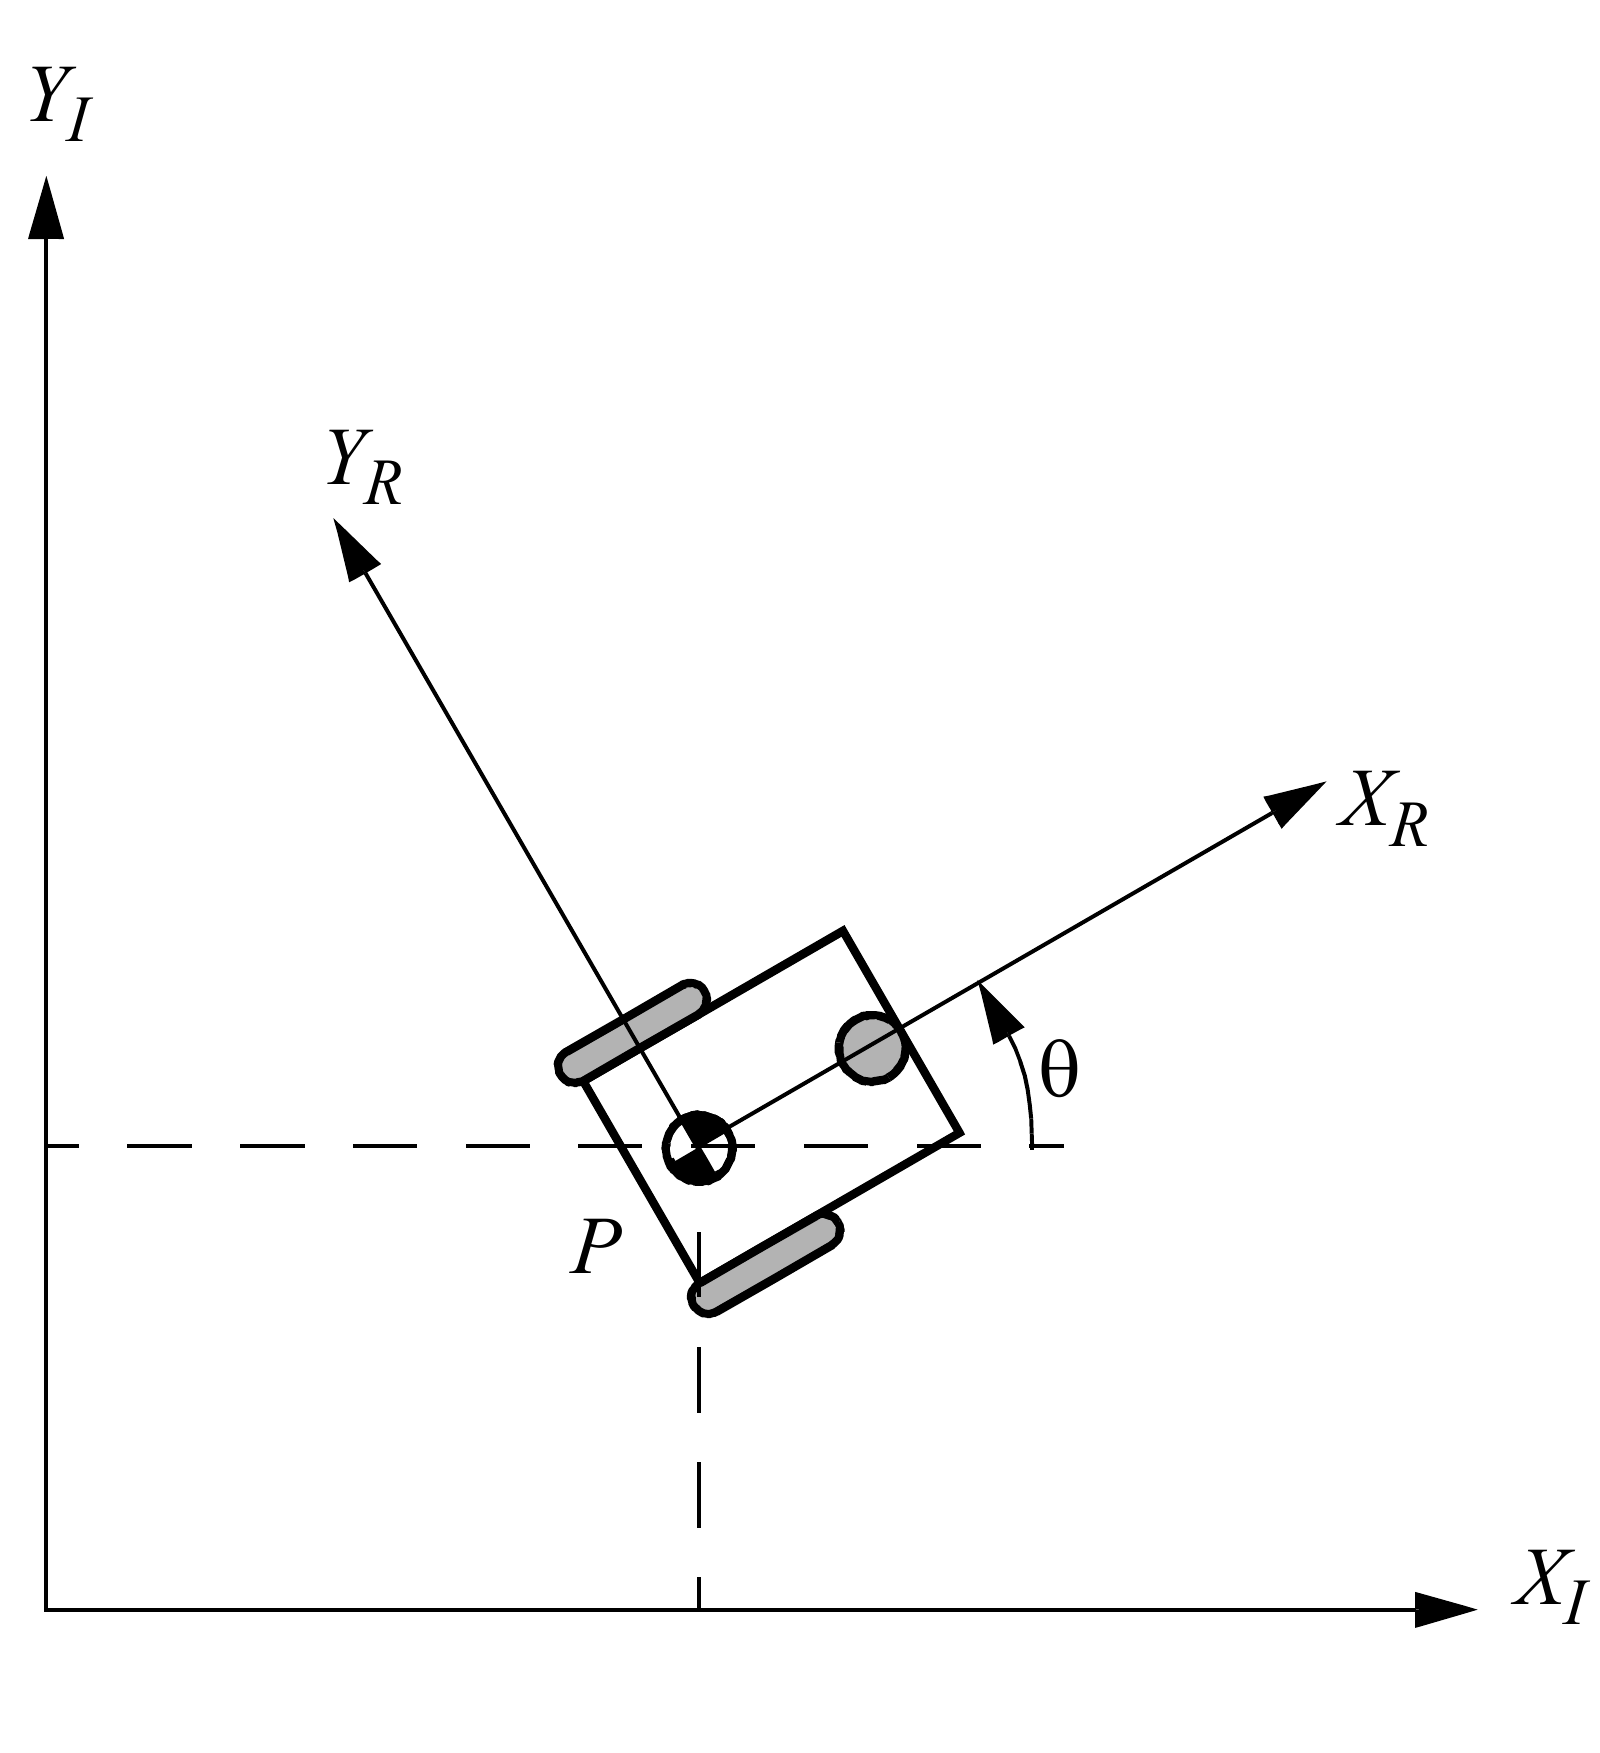
\includegraphics[width=\linewidth,height=4.5cm,keepaspectratio]{frames.png}
\caption{The global and robot coordinate frames.}
\end{figure}
\end{column}\begin{column}{.49\textwidth}
A \textbf{coordinate frame} is an origin plus axes.
\par\medskip Global frame $\{X_I,Y_I\}$: fixed to the world; $I$ means inertial.
\par\medskip Robot frame $\{X_R,Y_R\}$: attached at reference point $P$.
\[\xi_I=\begin{bmatrix}x&y&\theta\end{bmatrix}^{\mathsf T}\]
Pose $\xi_I$: position $(x,y)$ of $P$ and heading $\theta$ in the global frame. $\mathsf T$ denotes transpose.

\end{column}\end{columns}
\par\vspace{2mm}\small How do velocities convert between these frames?
\end{frame}

\begin{frame}[t]{Converting between the two frames}
\footnotesize
\vspace{0mm}
\begin{columns}[T,onlytextwidth]\begin{column}{.49\textwidth}
\[\dot\xi_R=R(\theta)\dot\xi_I\]
\[R(\theta)=\begin{bmatrix}\cos\theta&\sin\theta&0\\-\sin\theta&\cos\theta&0\\0&0&1\end{bmatrix}\]
\[\dot\xi_I=R(\theta)^{-1}\dot\xi_R=R(\theta)^{\mathsf T}\dot\xi_R\]
\footnotesize A dot means rate of change. $\dot\xi_I$ and $\dot\xi_R$ are the same velocity expressed in global and robot components. $R(\theta)$ rotates those components.

\end{column}\begin{column}{.49\textwidth}
\begin{figure}[H]\centering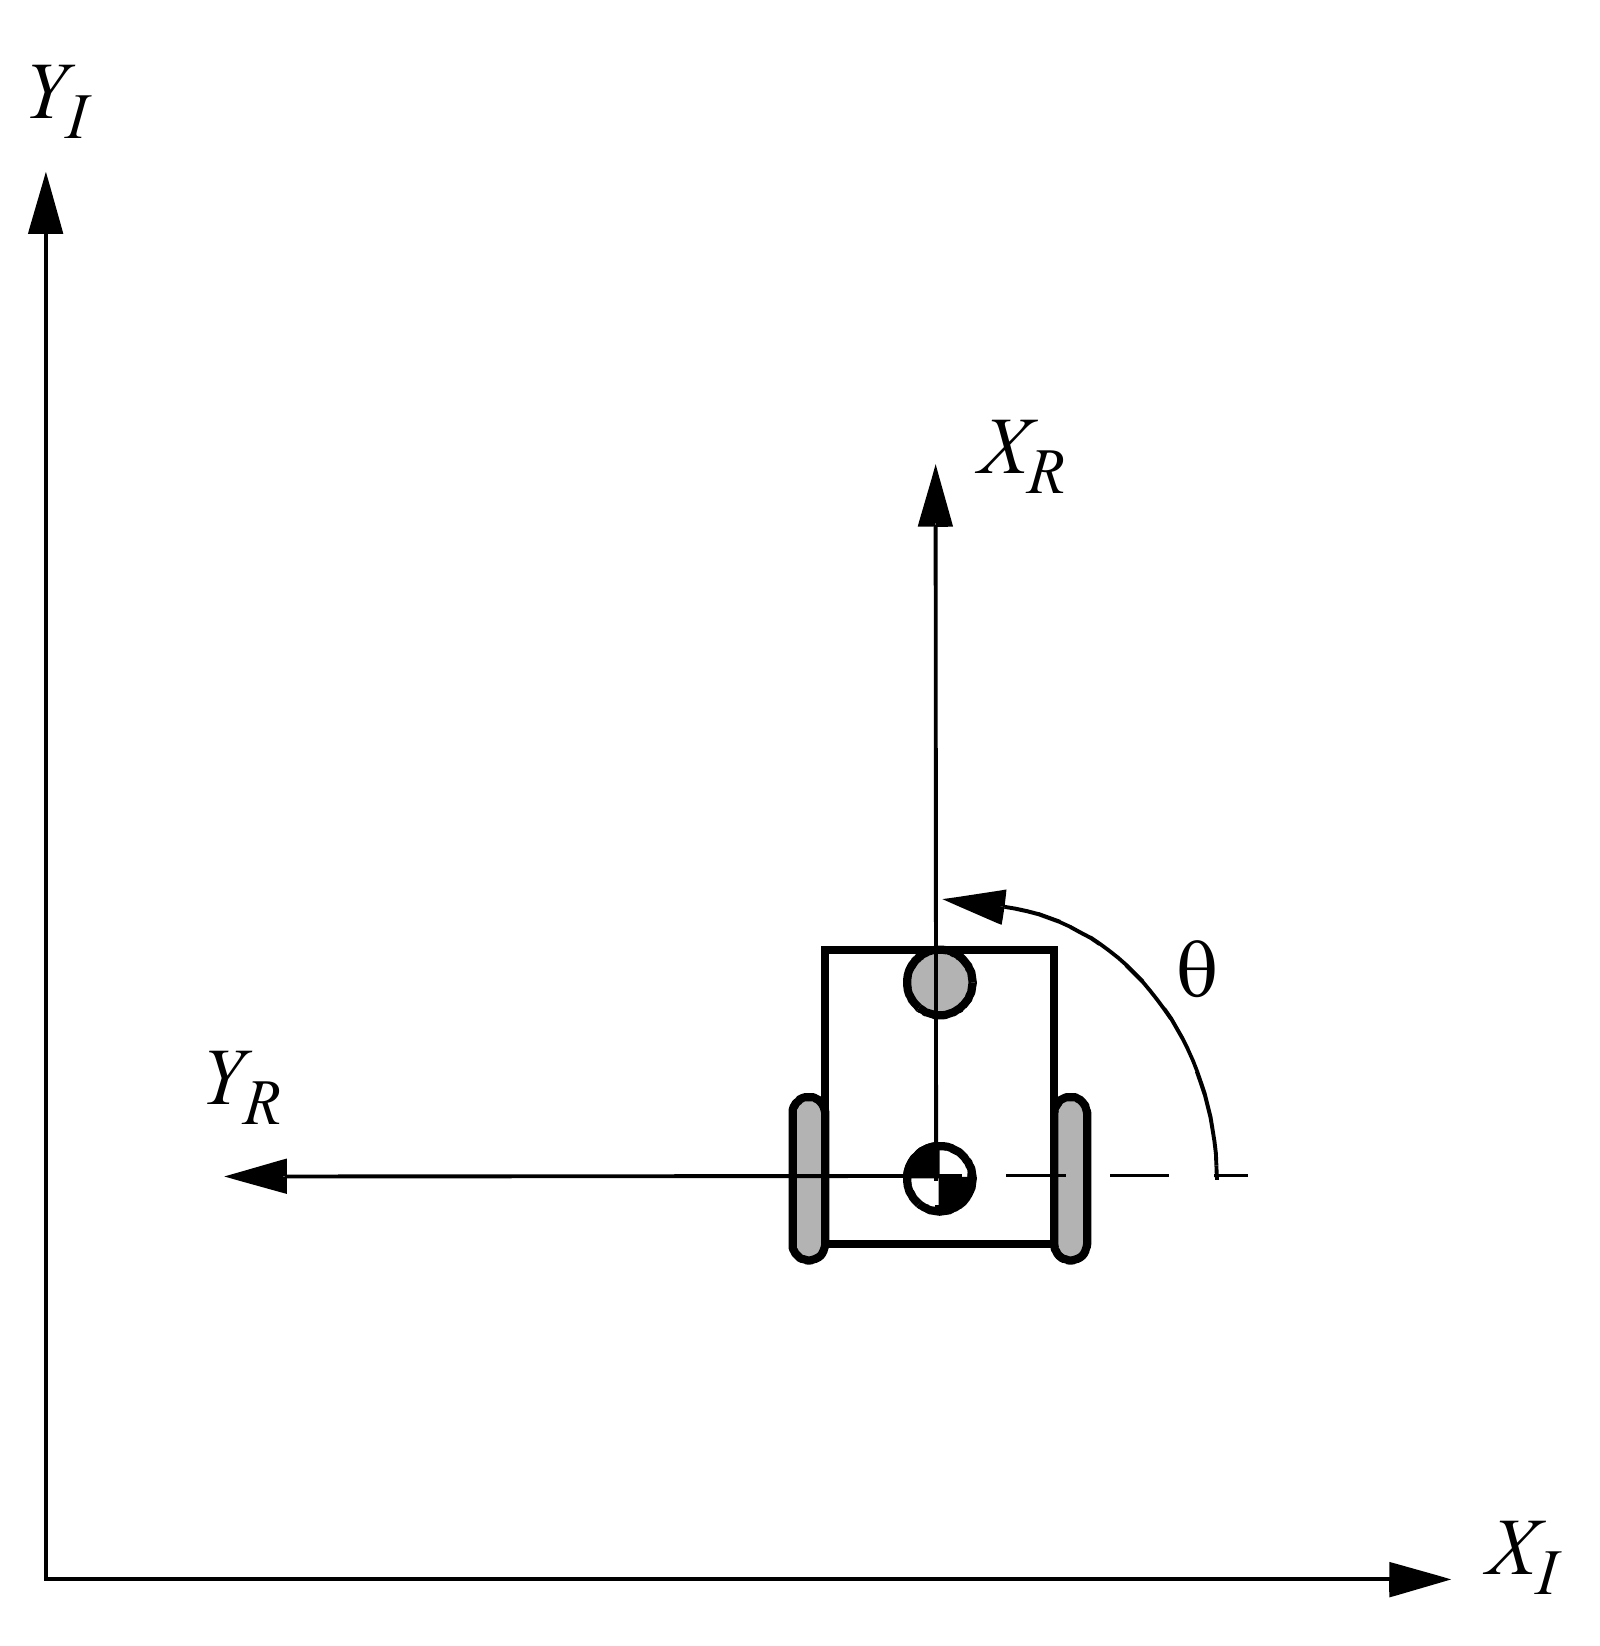
\includegraphics[width=\linewidth,height=4.1cm,keepaspectratio]{quarter_turn.png}
\caption{At $\theta=\pi/2$, robot forward is global $+Y_I$.}
\end{figure}\vspace{-3mm}\footnotesize Check: $\dot x_R=1$, $\dot y_R=0$ gives $\dot x_I=0$, $\dot y_I=1$.
\end{column}\end{columns}
\end{frame}

\begin{frame}[t]{What the robot measures and what we want}
\footnotesize
\vspace{-6mm}
\begin{columns}[T,onlytextwidth]\begin{column}{.49\textwidth}
\centering\begin{tikzpicture}[>=Latex,every node/.style={font=\small,align=center}]

\draw[thick] (0,0) circle (1);\draw[thick] (0,0)--(.7,.7);\foreach \a in {0,30,...,330}{\draw (\a:.85)--(\a:1);}\node at (0,-1.4) {Encoder: counts shaft rotation};\draw[->,blue] (1.4,0)--(3,0);\node[align=center] at (2.2,.8) {$\dot\varphi$\\rad/s};\node at (2.5,-.7) {$r\dot\varphi$\\m/s};

\end{tikzpicture}
\end{column}\begin{column}{.49\textwidth}
\begin{block}{Encoder}
A shaft sensor that counts ticks as the wheel turns. Changes in counts give how far and how fast it turns.
\end{block}
\vspace{3mm}
\footnotesize $r$: wheel radius. $\dot\varphi$: wheel angular speed. Under pure rolling, $r\dot\varphi$ is the wheel-centre speed along the wheel plane.\par\medskip Chassis forward kinematics maps wheel speeds to robot velocity. Odometry integrates that velocity into pose; wheel sensors alone do not directly measure global pose.
\end{column}\end{columns}
\par\vspace{2mm}\footnotesize Do this for the simplest chassis: two driven wheels.
\end{frame}

\begin{frame}[t]{Differential drive: each wheel adds its own part}
\small
\vspace{-6mm}
\begin{columns}[T,onlytextwidth]\begin{column}{.49\textwidth}
\centering
\begin{tikzpicture}[scale=1,>=Latex]
\draw[rounded corners] (-.8,-1.25) rectangle (1.4,1.25);
\draw[very thick] (-.4,-1)--(.4,-1);\draw[very thick] (-.4,1)--(.4,1);
\fill[blue] (0,0) circle (2pt) node[below right] {$P$};
\draw[->] (0,0)--(2.1,0) node[right] {$X_R$};\draw[->] (0,0)--(0,1.8) node[above] {$Y_R$};
\draw[<->] (-1.05,0)--(-1.05,-1) node[midway,left] {$l$};
\node[below] at (0,-1.3) {\small 1 (right), $\dot\varphi_1$};
\node[above right] at (.4,1.25) {\small 2 (left), $\dot\varphi_2$};
\end{tikzpicture}
\par\small $l$: half the distance between wheels.\\ $r$: wheel radius. $\dot\varphi_1$: right wheel; $\dot\varphi_2$: left wheel angular speed.
\end{column}\begin{column}{.49\textwidth}
\[\dot x_R=\frac r2(\dot\varphi_1+\dot\varphi_2),\quad\dot y_R=0\]
\[\dot\theta=\frac r{2l}(\dot\varphi_1-\dot\varphi_2)\]
\[\dot\xi_I=R(\theta)^{-1}\begin{bmatrix}r(\dot\varphi_1+\dot\varphi_2)/2\\0\\r(\dot\varphi_1-\dot\varphi_2)/(2l)\end{bmatrix}\]
\small Equal speeds: straight. Opposite speeds: spin in place. If wheel 1 is faster, which way does the robot turn?

\end{column}\end{columns}
\par\vspace{2mm}\small See the same command on three bases.
\end{frame}

\begin{frame}[t]{Demo 1: one command, three robots, then noise}
\small
\vspace{-3mm}
\begin{figure}[H]
\centering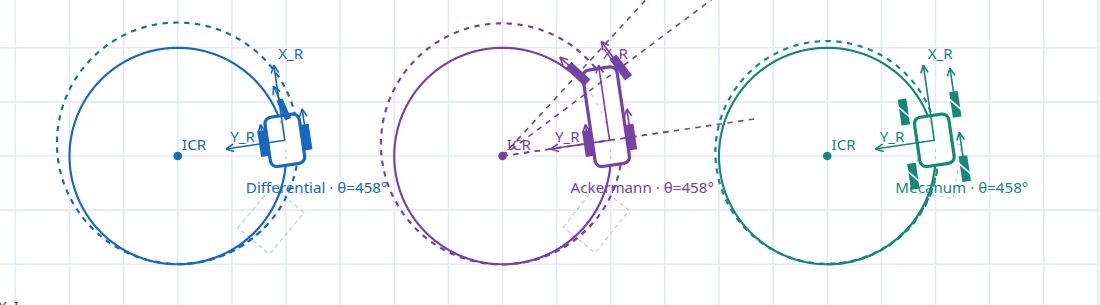
\includegraphics[width=\textwidth,keepaspectratio]{demo_drift.png}
\caption{True paths (solid) and odometry (dashed), with encoder noise.}
\end{figure}
\footnotesize
Set $v=0.4$ m/s, $\omega=0.4$ rad/s, then enable encoder noise. Odometry = pose from integrating wheel speeds; errors accumulate. What does a wheel forbid?
\end{frame}

\begin{frame}[t]{What a wheel forbids}
\small
\vspace{-6mm}
\begin{columns}[T,onlytextwidth]\begin{column}{.49\textwidth}
\begin{figure}[H]\centering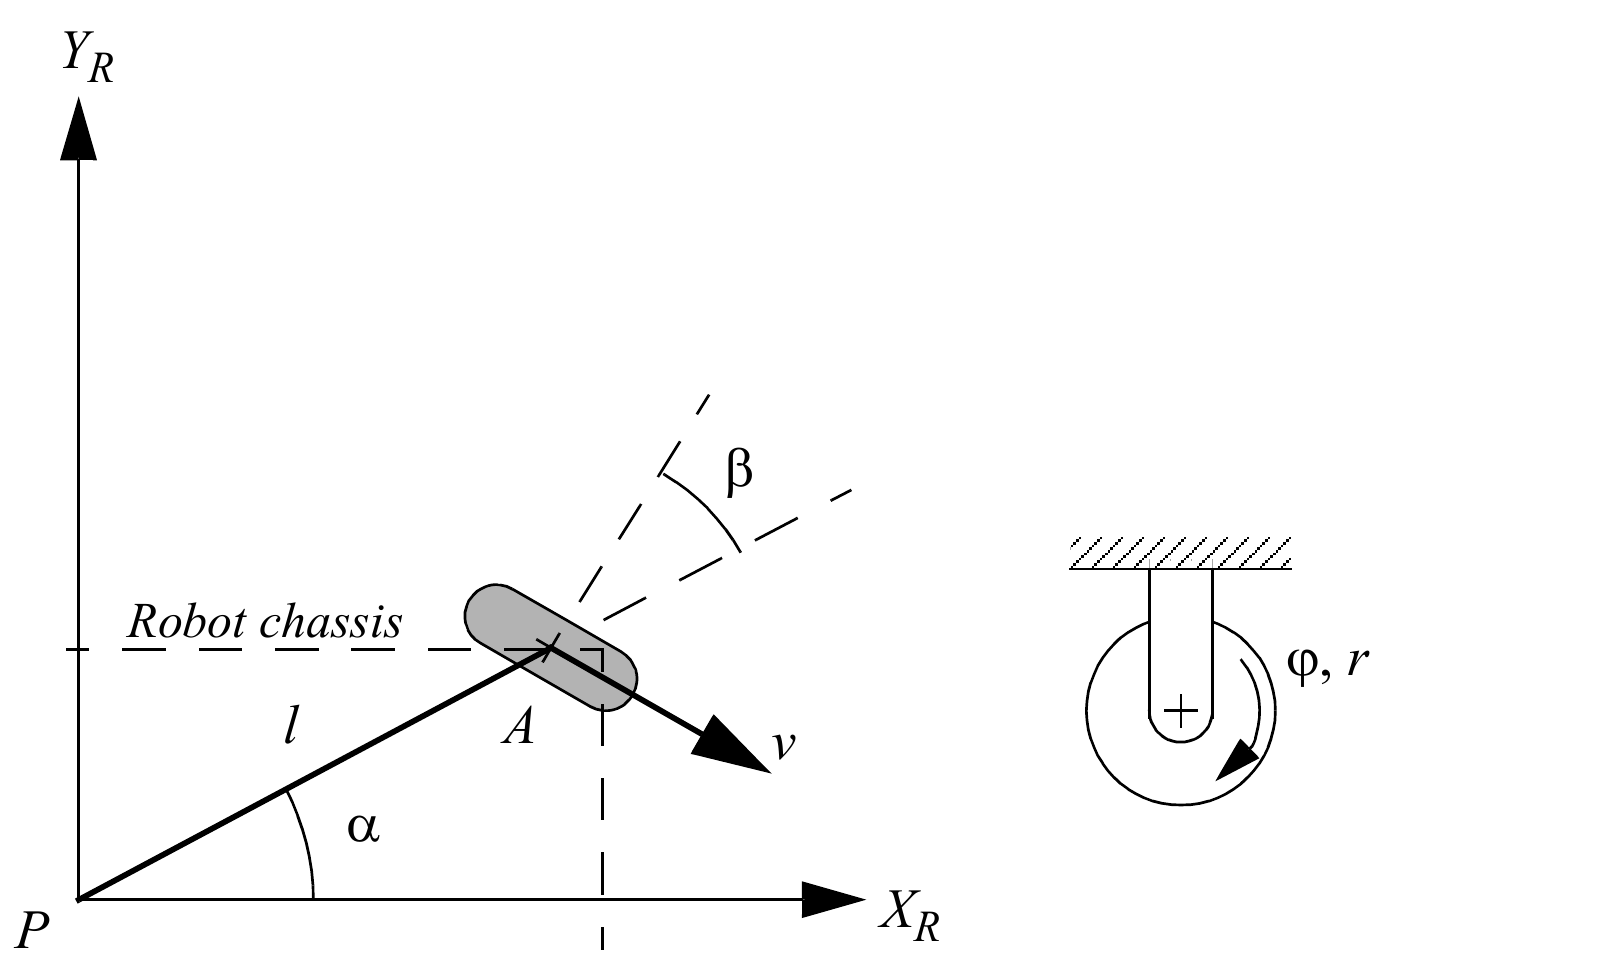
\includegraphics[width=\linewidth,height=4.5cm,keepaspectratio]{fixed.png}
\caption{A fixed wheel at point A, relative to reference point P.}
\end{figure}
\end{column}\begin{column}{.49\textwidth}
\small $l=|PA|$: distance from $P$ to the wheel. $\alpha$: angle of $PA$ from $X_R$. $\beta$: wheel-axis angle relative to $PA$. $r$: wheel radius; $\varphi$: wheel rotation.
\par\medskip Rolling: velocity along the wheel plane matches $r\dot\varphi$.
\par\medskip No sideways slip: the lateral contact velocity is zero. Under pure rolling, the material contact point is instantaneously stationary relative to the ground.

\end{column}\end{columns}
\par\vspace{2mm}\small Write both requirements as equations.
\end{frame}

\begin{frame}[t]{The two equations of a fixed wheel}
\small
\vspace{-3mm}
\begin{block}{Rolling along the wheel plane}
\[\begin{bmatrix}\sin(\alpha+\beta)&-\cos(\alpha+\beta)&-l\cos\beta\end{bmatrix}R(\theta)\dot\xi_I-r\dot\varphi=0\]
The chassis velocity at the wheel matches its rolling speed.

\end{block}
\vspace{3mm}
\begin{block}{No sliding across the wheel plane}
\[\begin{bmatrix}\cos(\alpha+\beta)&\sin(\alpha+\beta)&l\sin\beta\end{bmatrix}R(\theta)\dot\xi_I=0\]
The wheel cannot move sideways under the no-slip assumption.

\end{block}
\par\vspace{2mm}\small How do other wheel types change these constraints?
\end{frame}

\begin{frame}[t]{The other wheels in one table}
\small
\vspace{0mm}
\begin{tabularx}{\linewidth}{lXXX}
\toprule Wheel & Fixed / free & Rolling & Sideways constraint\\\midrule
Steered & Controlled $\beta(t)$ & Same form & Same form at current angle\\
Castor & Free swivel; offset & Same form & Extra swivel-rate term\\
Swedish & Free roller & Roller angle enters & Roller motion absorbs lateral speed\\
Spherical & Free rolling direction & Direction follows motion & No chassis restriction\\\bottomrule
\end{tabularx}
\par\vspace{3mm}\small Castor: $d$ is steering offset; $\dot\beta$ is free swivel rate and can satisfy the sideways equation.
\[\begin{bmatrix}\cos(\alpha+\beta)&\sin(\alpha+\beta)&d+l\sin\beta\end{bmatrix}R(\theta)\dot\xi_I+d\dot\beta=0\]


\par\vspace{2mm}\small How are the constraints of several wheels combined?
\end{frame}

\begin{frame}[t]{From wheels to the robot}
\small
\vspace{-2mm}
\begin{block}{Stack the rolling equations}
\[J_1(\beta_s)R(\theta)\dot\xi_I-J_2\dot\varphi=0\]
$J_1$: rolling projections; $J_2$: diagonal wheel radii; $\dot\varphi$: wheel-rate vector.

\end{block}
\vspace{3mm}
\begin{block}{Stack the no-sideways-slip equations}
\[C_1(\beta_s)R(\theta)\dot\xi_I=0\]
$C_1$: sliding constraints; $\beta_s$: steering angles. Fixed rows are constant; steered rows vary.

\end{block}
\par\vspace{2mm}\small Use the equations on the differential drive first.
\end{frame}

\begin{frame}[t]{Example: differential drive}
\small
\vspace{-6mm}
\begin{columns}[T,onlytextwidth]\begin{column}{.49\textwidth}
\centering
\begin{tikzpicture}[scale=1,>=Latex]
\draw[rounded corners] (-.8,-1.25) rectangle (1.4,1.25);
\draw[very thick] (-.4,-1)--(.4,-1);\draw[very thick] (-.4,1)--(.4,1);
\fill[blue] (0,0) circle (2pt) node[below right] {$P$};
\draw[->] (0,0)--(2.1,0) node[right] {$X_R$};\draw[->] (0,0)--(0,1.8) node[above] {$Y_R$};
\draw[<->] (-1.05,0)--(-1.05,-1) node[midway,left] {$l$};
\node[below] at (0,-1.3) {\small 1 (right), $\dot\varphi_1$};
\node[above right] at (.4,1.25) {\small 2 (left), $\dot\varphi_2$};
\end{tikzpicture}\par\small ICR: instantaneous rotation centre. If $\omega\ne0$, $\mathrm{ICR}_R=(0,v/\omega)$, on the common axle.


\end{column}\begin{column}{.49\textwidth}
Two rolling equations; one independent lateral constraint:
\[\begin{bmatrix}1&0&l\\1&0&-l\\0&1&0\end{bmatrix}\dot\xi_R=\begin{bmatrix}r\dot\varphi_1\\r\dot\varphi_2\\0\end{bmatrix}\]
\[\dot\xi_R=\begin{bmatrix}r(\dot\varphi_1+\dot\varphi_2)/2\\0\\r(\dot\varphi_1-\dot\varphi_2)/(2l)\end{bmatrix}\]
\small \par For straight travel, the ICR is at infinity.

\end{column}\end{columns}
\par\vspace{2mm}\small What changes when each wheel has a free roller?
\end{frame}

\begin{frame}[t]{Example: omnidirectional robot (three Swedish wheels)}
\small
\vspace{-1mm}
$C_1$ empty; $J_1$ invertible: $\dot\xi_I=R(\theta)^{-1}J_1^{-1}J_2\dot\varphi$.
\begin{columns}[T,onlytextwidth]\begin{column}{.49\textwidth}
\begin{figure}[H]\centering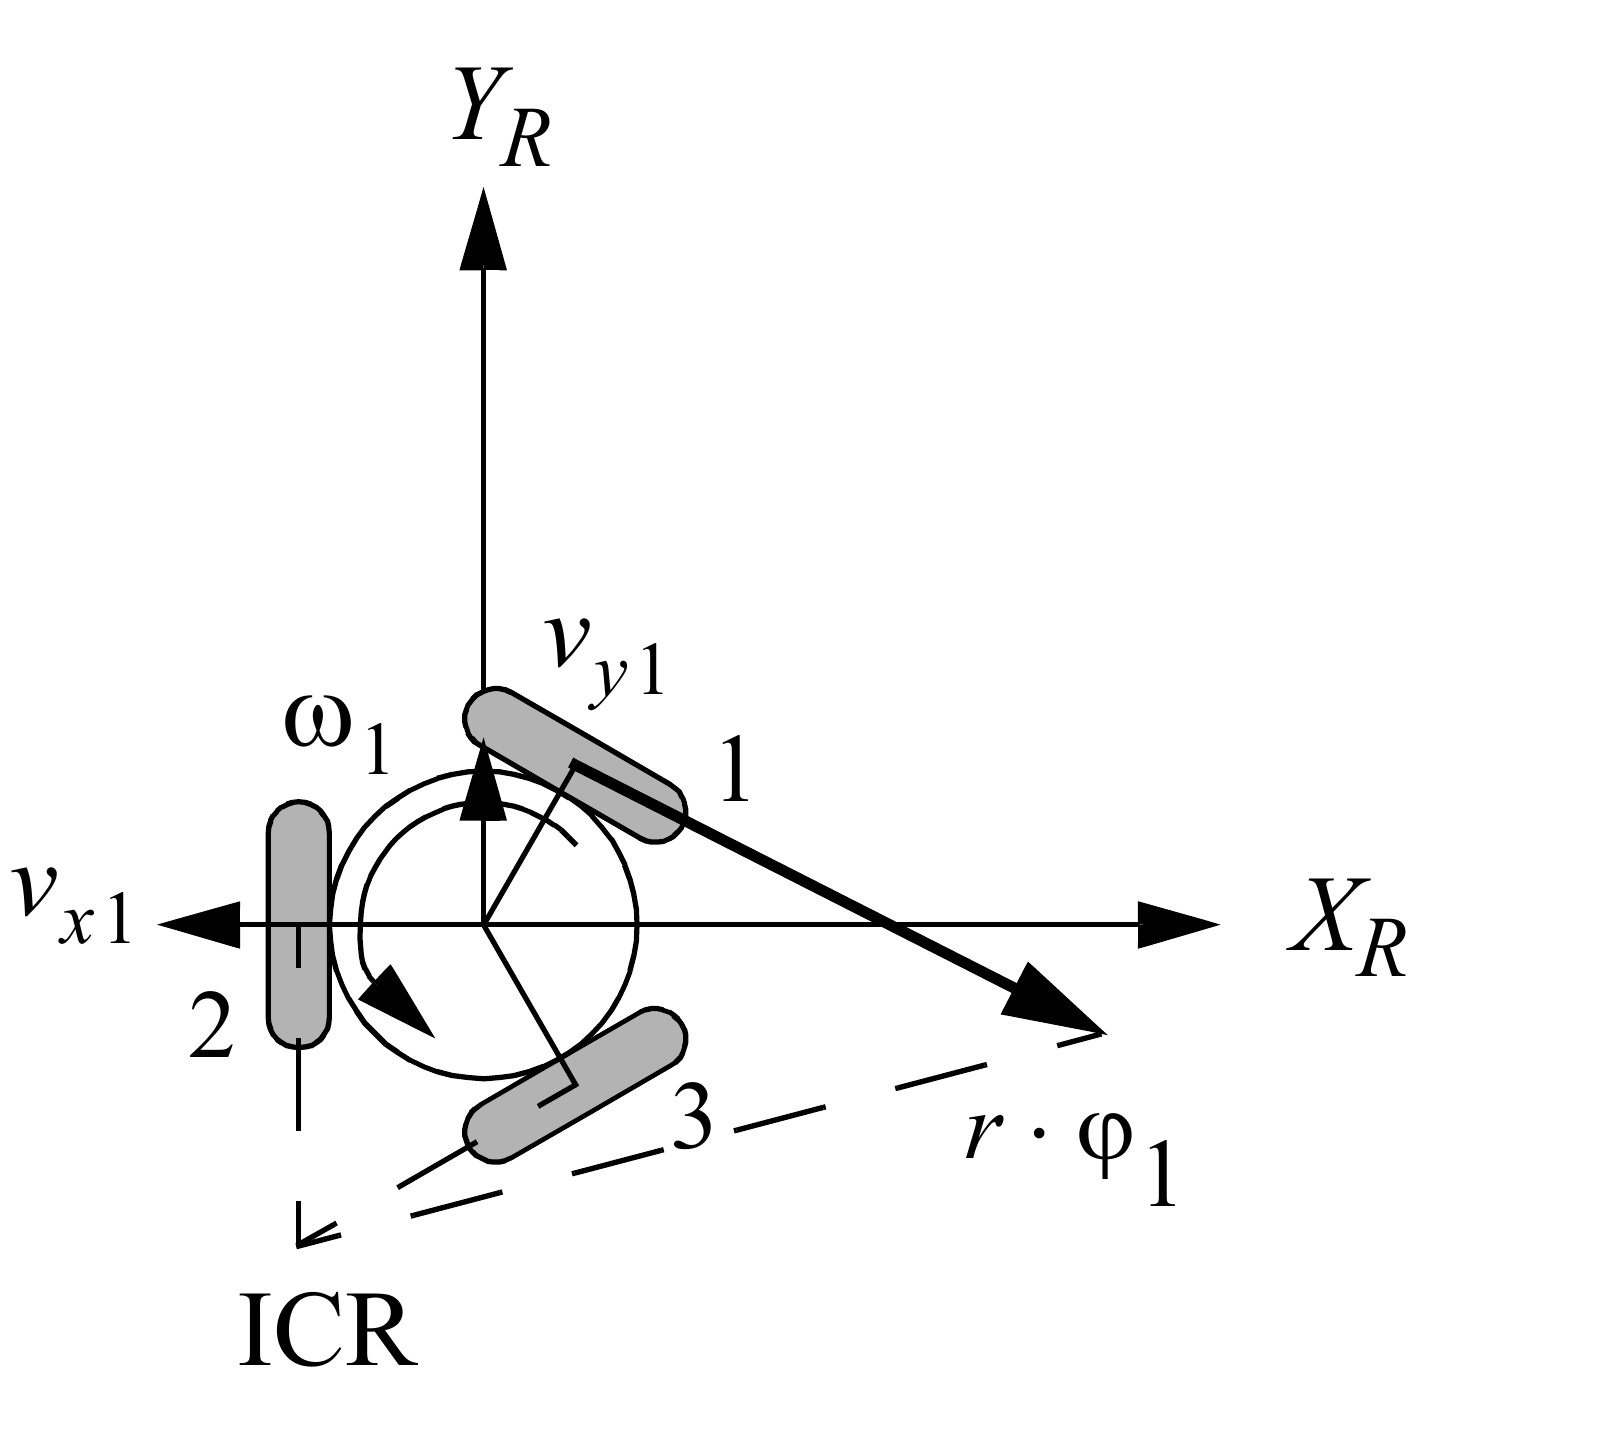
\includegraphics[width=\linewidth,height=4.5cm,keepaspectratio]{omni_geometry.png}
\caption{Three free velocity components.}
\end{figure}
\end{column}\begin{column}{.49\textwidth}
\begin{figure}[H]\centering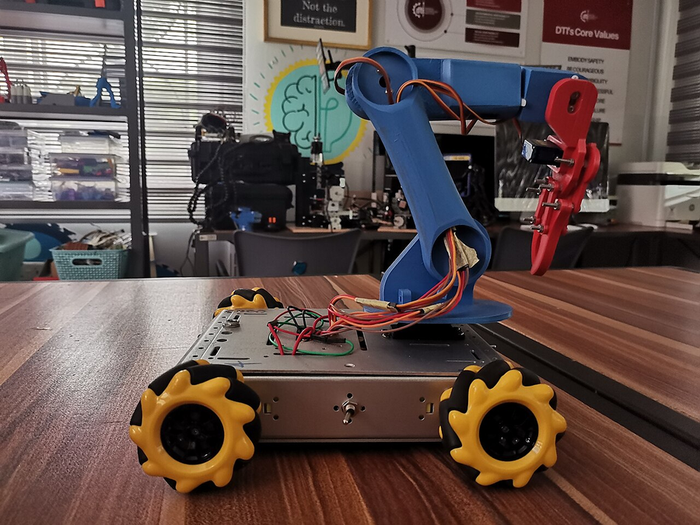
\includegraphics[width=\linewidth,height=4.5cm,keepaspectratio]{mecanum.png}
\caption{A mecanum platform with free rollers.}
\end{figure}
\end{column}\end{columns}
\end{frame}

\begin{frame}[t]{Degree of mobility}
\small
\vspace{-1mm}
\begin{columns}[T,onlytextwidth]\begin{column}{.49\textwidth}
\begin{figure}[H]\centering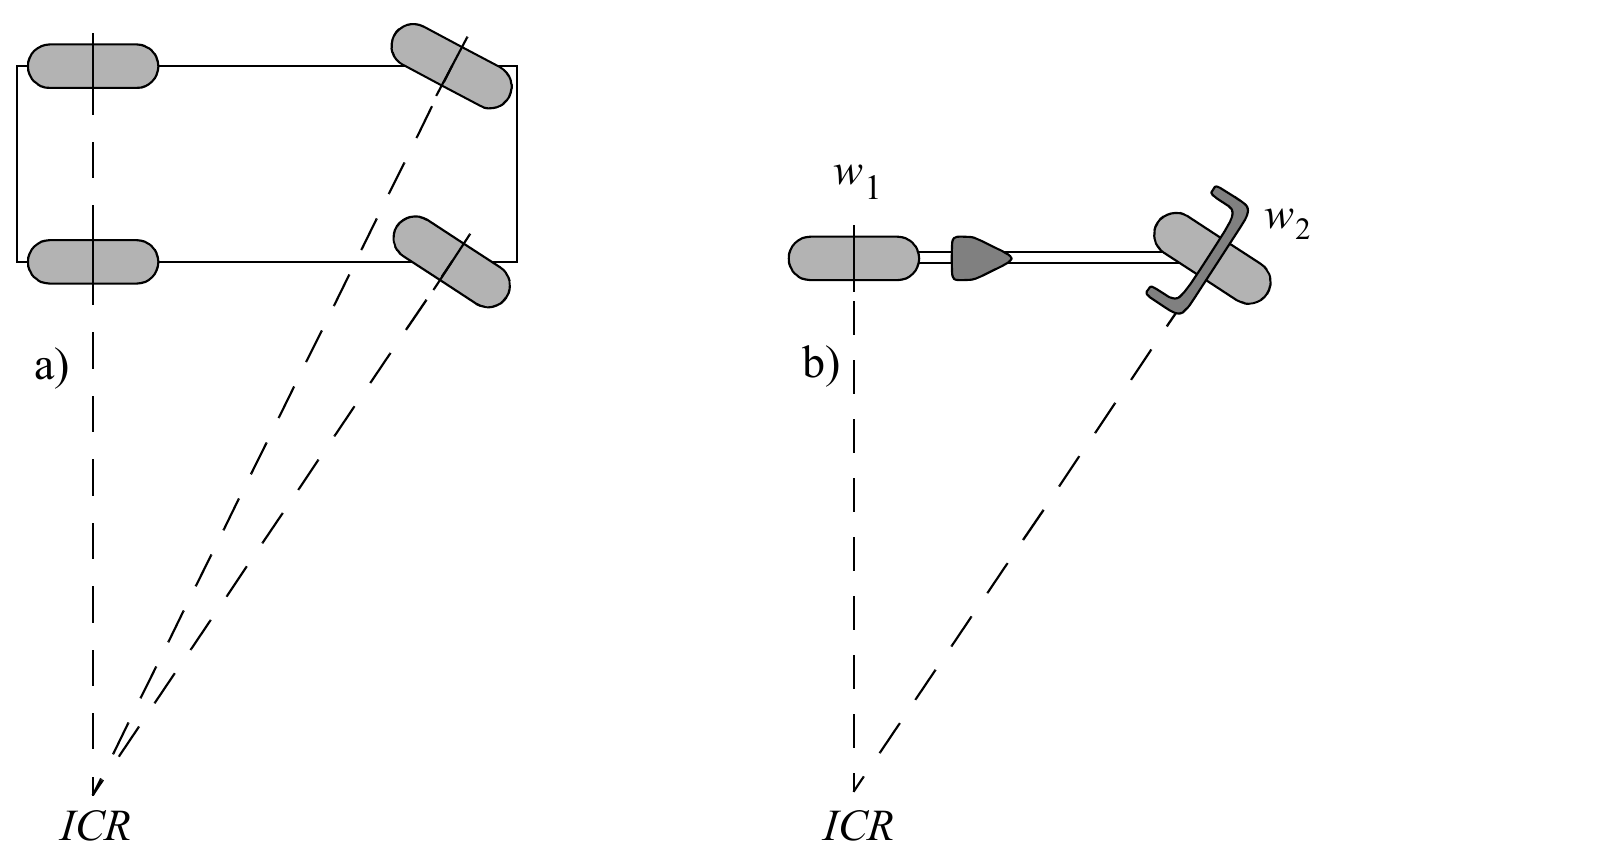
\includegraphics[width=\linewidth,height=4.5cm,keepaspectratio]{ack_icr.png}
\caption{Wheel axes constrain the instantaneous rotation centre.}
\end{figure}
\end{column}\begin{column}{.49\textwidth}

\[\begin{aligned}\delta_m&=\dim\mathcal N(C_1(\beta_s))\\&=3-\operatorname{rank}C_1(\beta_s)\end{aligned}\]
\small $\mathcal N$: allowed velocities (null space); $\dim$: dimension. Rank counts independent constraints. Steering is held fixed.


\begin{tabular}{lcc}Base & Rank & $\delta_m$\\\hline Differential & 1 & 2\\ Ackermann & 2 & 1\\ Omni & 0 & 3\end{tabular}
\end{column}\end{columns}
\par\vspace{2mm}\small How does steering add capability?
\end{frame}

\begin{frame}[t]{Steerability and manoeuvrability}
\small
\vspace{-6mm}
\begin{columns}[T,onlytextwidth]\begin{column}{.49\textwidth}
\begin{figure}[H]\centering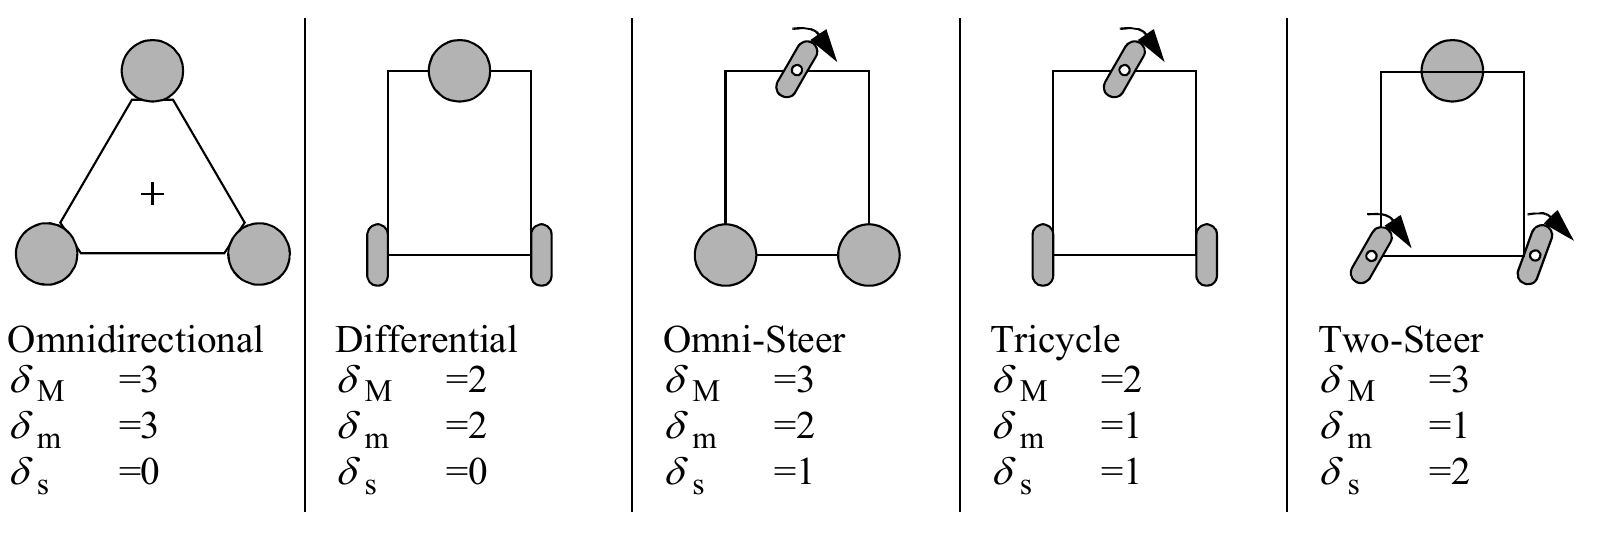
\includegraphics[width=\linewidth,height=4.5cm,keepaspectratio]{five_classes.png}
\caption{Five basic wheel arrangements.}
\end{figure}
\end{column}\begin{column}{.49\textwidth}
\begin{block}{Steerability and manoeuvrability}
$\delta_s$: number of independent steering freedoms, respecting steering linkages.\\ $\delta_M=\delta_m+\delta_s$: degree of manoeuvrability.
\end{block}
\vspace{3mm}
\begin{tabular}{lccc}
Base & $\delta_m$ & $\delta_s$ & $\delta_M$\\\hline
Differential & 2 & 0 & 2\\
Ackermann & 1 & 1 & 2\\
Omni & 3 & 0 & 3
\end{tabular}
\par\medskip\small Steering changes allowed motion. Subsequent travel changes the pose.

\end{column}\end{columns}
\par\vspace{2mm}\small Which base is easier to park sideways?
\end{frame}

\begin{frame}[t]{Demo 2: park sideways by one metre}
\small
\vspace{-3mm}
\begin{figure}[H]
\centering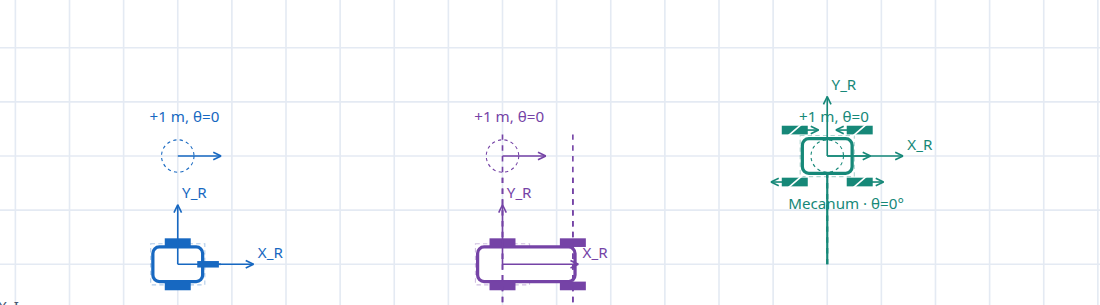
\includegraphics[width=\textwidth,keepaspectratio]{demo_parking.png}
\caption{Only the mecanum base follows a sideways command.}
\end{figure}
\footnotesize
Differential: turn, drive, turn back. Ackermann: forward and reverse arcs. Omni: one straight segment. What should we keep from the lecture?
\end{frame}

\begin{frame}[t]{What to remember}
\small
\vspace{-3mm}
\begin{block}{1. Locomotion is a design trade-off}
Stability, contact, environment: legs select footholds; wheels suit hard, flat ground.
\end{block}
\vspace{3mm}
\begin{block}{2. Wheel speeds give velocity; velocity integrates to pose}
Use the global and robot frames consistently. Rolling constraints connect wheel rates to motion; sliding constraints restrict it.
\end{block}
\vspace{3mm}
\begin{block}{3. Mobility and steering are different freedoms}
$\delta_m$: instantaneous mobility. $\delta_s$: independent steering. $\delta_M$: their sum.
\end{block}
\vspace{3mm}
\small Next lecture: workspace, holonomic constraints, path versus trajectory, feedback.
\end{frame}

\begin{frame}[t]{Reference Materials}
    \begin{itemize}
        \item Siegwart, Nourbakhsh, Scaramuzza --- Siegwart Nourbakhsh Scaramuzza Introduction to Autonomous Mobile Robots Second Edition
        \item Auledas --- ANYmal on rough ground, CC BY-SA 4.0
        \item Daderot --- RHex robotic hexapod, CC0
        \item Jonte --- Spot quadruped robot, CC BY-SA 4.0
        \item GearSkeptic --- Rocker-bogie model, CC0
        \item Anani A. George --- Mecanum wheel robot, CC0
    \end{itemize}
\end{frame}

\fbckg{fibeamer/figs/last_page.png}
\frame[plain]{}

\end{document}
